%!TEX TS-program = pdflatex
%!TEX encoding = UTF-8 Unicode
% =============================================================================
%  P1_bernoulli.tex   --  Bernoulli submission version
%  Compile order:
%    (1) pdflatex P1_bernoulli_supp.tex   (twice)
%    (2) pdflatex P1_bernoulli.tex
%    (3) bibtex   P1_bernoulli
%    (4) pdflatex P1_bernoulli.tex  (twice)
% =============================================================================
\documentclass[bj,authoryear]{imsart}

\usepackage{amsmath,amssymb,mathtools}
\usepackage{bm}
\usepackage{booktabs}
\usepackage{array}
\usepackage{multirow}
\usepackage{enumitem}
\usepackage{graphicx}
\usepackage{float}
\usepackage[section]{placeins}
\usepackage{microtype}
% ── Local definitions (theorem environments + math macros) ───────────────────
\startlocaldefs
\emergencystretch=2em

\theoremstyle{plain}
\newtheorem{theorem}{Theorem}[section]
\newtheorem{proposition}[theorem]{Proposition}
\newtheorem{lemma}[theorem]{Lemma}
\newtheorem{corollary}[theorem]{Corollary}
\theoremstyle{definition}
\newtheorem{definition}[theorem]{Definition}
\newtheorem{example}[theorem]{Example}
\newtheorem{remark}[theorem]{Remark}
\newtheorem{assumption}[theorem]{Assumption}

\newcommand{\E}{\mathbb{E}}
\newcommand{\Prob}{\mathbb{P}}
\newcommand{\R}{\mathbb{R}}
\newcommand{\N}{\mathbb{N}}
\newcommand{\F}{\mathcal{F}}
\newcommand{\G}{\mathcal{G}}
\newcommand{\A}{\mathcal{A}}
\newcommand{\Z}{\mathcal{Z}}
\newcommand{\Tsig}{\mathcal{T}_\infty}
\newcommand{\norm}[1]{\left\lVert #1 \right\rVert}
\newcommand{\abs}[1]{\left| #1 \right|}
\newcommand{\inner}[2]{\langle #1,\, #2 \rangle}
\newcommand{\given}{\mid}
\newcommand{\iid}{\overset{\mathrm{iid}}{\sim}}
\DeclareMathOperator{\Var}{Var}
\DeclareMathOperator{\Cov}{Cov}
\DeclareMathOperator*{\argmin}{arg\,min}
\newcommand{\od}[1]{\overset{d}{#1}}

\endlocaldefs

% Cross-references to Supplementary Material (inlined from P1_supp_xrefs.tex)
\makeatletter
\expandafter\def\csname r@app:background\endcsname{{A}{1}{Background and Preliminaries}{section.1}{}}
\expandafter\def\csname r@app:proofs\endcsname{{B}{4}{Proofs}{section.2}{}}
\expandafter\def\csname r@app:sims\endcsname{{C}{4}{Simulation Details}{section.3}{}}
\expandafter\def\csname r@app:stationary-causal\endcsname{{B.9}{}{Stationary Causal Solution and Geometric Coupling}{subsection.2.9}{}}
\expandafter\def\csname r@app:supp-empirical\endcsname{{D}{}{Empirical Supplement}{section.4}{}}
\expandafter\def\csname r@app:supp-lsdiag\endcsname{{D.1}{}{Study LS-Diag: Locally Stationary AR}{subsection.4.1}{}}
\expandafter\def\csname r@app:supp-jsurr\endcsname{{D.2}{}{Study J-Surr: $J_t$ Surrogate Comparison}{subsection.4.2}{}}
\makeatother

% =============================================================================
\begin{document}

\begin{frontmatter}

\title{Martingale Innovations from Contractive Recurrent Networks
       and Dimension-Robust Change-Point Detection}
\runtitle{Martingale Innovations and Dimension-Robust Detection}

\author{\inits{Y.-C.\,I.}\fnms{Yuan-chin Ivan}~\snm{Chang}%
  \ead[label=e1]{ycchang@stat.sinica.edu.tw}}
\address{Institute of Statistical Science, Academia Sinica,
  128 Academia Road, Section~2, Nankang, Taipei 115, Taiwan.
  \printead[presep={\ }]{e1}}

\begin{abstract}
Recurrent neural networks (RNNs) are widely used for sequential data, yet a basic question remains open:
what does the hidden state of a trained RNN actually encode about its input
sequence?
A related gap affects change-point detection: standard cumulative sum (CUSUM)
procedures assume independent or parametrically specified input, and their
false-alarm guarantees break down when the serial dependence is unknown or
the observation dimension is large.

This paper addresses both gaps.
We establish that the hidden state of a contractive RNN decomposes, at every
step, into a predictable component and an innovation that satisfies the
martingale-difference property; under mild conditions the accumulated innovations
satisfy a functional central limit theorem.
Building on this, we introduce the Innovation CUSUM, which applies a CUSUM
statistic to LSTM prediction innovations.
Because these innovations are approximately free of serial dependence by
construction, the detector's false-alarm rate remains well-controlled as the
observation dimension grows, without requiring knowledge of the dependence
structure.

Eight empirical studies on synthetic and real data support the theory.
Applications to the Nile River discharge series and US equity sector returns
around the 2020 COVID crash are consistent with the theoretical predictions.

\end{abstract}

\begin{keyword}
\kwd{martingale decomposition}
\kwd{recurrent neural network}
\kwd{LSTM}
\kwd{change-point detection}
\kwd{CUSUM}
\kwd{average run length}
\kwd{dimension stability}
\kwd{locally stationary processes}
\end{keyword}

\end{frontmatter}

\section{Introduction}
\label{sec:intro}

Sequential data arise throughout science and engineering: physiological signals in
intensive care, infectious disease incidence, machinery sensor streams.  In each
setting the central question is the same --- how much of the past is relevant to
the present?  Classical time-series models answer this parametrically.
Autoregressive models fix the lag order; hidden Markov models encode memory
through a finite state space; Kalman filters propagate a Gaussian sufficient
statistic \citep{box2015time, hamilton1994time}.  Each framework carries an
explicit probabilistic account of what is remembered.

Deep sequential architectures aspire instead to learn the relevant memory horizon
from data.  Recurrent neural networks (RNNs) \citep{rumelhart1986learning}, long short-term
memory networks (LSTMs) \citep{hochreiter1997long}, gated recurrent units
(GRUs) \citep{cho2014learning}, and selective state-space models (SSMs)
such as Mamba \citep{gu2023mamba} implement increasingly
sophisticated gating mechanisms for this purpose.  Yet a fundamental asymmetry
persists: the empirical performance of these architectures is well documented,
while the probabilistic account of what they retain is almost entirely absent.
What does a trained LSTM encode in its cell state?  What does the forget gate
actually discard?

The probabilistic object formalizing what survives after any finite prefix is
the \emph{tail $\sigma$-algebra} $\Tsig=\bigcap_{n\geq1}\sigma(X_n,X_{n+1},\ldots)$;
Theorem~\ref{thm:mds} makes this framing rigorous for contractive RNNs.

The natural tool is reverse martingale theory
\citep{doob1953stochastic,williams1991probability}: sequences adapted to a
decreasing filtration converge automatically in both almost-sure and $L^1$
senses, the rigorous backbone of our proofs.

This paper establishes four results connecting this classical theory to
recurrent architectures and change-point detection.
%
The first result shows that, under a contraction condition on the recurrent
weight matrix (Assumption~\ref{ass:spectral}), the hidden state splits at
every step into a component fully determined by the past and a genuinely new
component that carries only the fresh information in the current observation.
This new component stabilizes geometrically and has a non-degenerate variance
structure (Theorem~\ref{thm:mds}); the stationary causal solution used as
background is established in \citet{chang2026jrssb}.
%
The second result shows that the accumulated new-information components,
suitably normalized, converge in distribution to a Brownian motion,
providing the asymptotic theory needed to calibrate inference procedures
built on these innovations (Corollary~\ref{cor:fclt}).

The third and fourth results concern change-point detection.
We prove that a cumulative sum (CUSUM) detector built on LSTM prediction
innovations --- which inherit the new-information property above ---
has a false-alarm rate that is exponentially controlled in the detection
threshold, and that this guarantee remains stable as the observation
dimension grows (Theorem~\ref{thm:arl} and Corollary~\ref{cor:dim}).
Two supporting results underpin the main theorems: a lemma on the
equivalence of forward and reverse filtration limits, and a proposition
establishing that exact Bayes prediction residuals carry no predictable
component (Lemma~\ref{lem:equiv} and Proposition~\ref{prop:predresid}).

Existing work on recurrent architectures addresses stability
and expressibility \citep{miller2019stable,miyato2018spectral,gonon2020reservoir}
rather than the informational content of the hidden state.
The neural tangent kernel \citep{jacot2018neural} and information bottleneck
\citep{tishby2015deep,saxe2019information} frameworks apply to feedforward
networks or to compression at a fixed time step, not to sequential memory.
Structured state-space models and Mamba \citep{gu2021efficiently,gu2023mamba}
have been studied mainly for computational efficiency
\citep{orvieto2023resurrecting}.
On the detection side, standard CUSUM \citep{page1954continuous,lorden1971procedures},
offline segmentation \citep{killick2012optimal}, and Bayesian online
methods \citep{adams2007bayesian} are calibrated for independent or fully
specified parametric input and lose their guarantees under unknown serial
dependence or growing dimension.
Reverse martingale convergence is classical
\citep{doob1953stochastic,neveu1975discrete,hall1980martingale} but
its application to learned sequential architectures appears unexplored.
The non-stationary extension uses the locally stationary framework of
\citet{dahlhaus1997fitting}.

The theoretical framework and main results appear in
Sections~\ref{sec:theory}--\ref{sec:pathway}, followed by eight empirical
studies in Section~\ref{sec:empirical}.
Background definitions and all formal proofs are given in the Appendices
and Supplementary Material.

% =============================================================================
\section{Methodology}
\label{sec:theory}

%\subsection*{Setup}

We work on a complete probability space $(\Omega, \mathcal{A}, \mathbb{P})$.
Let $(X_t)_{t\geq 1}$ be a strictly stationary ergodic process with natural
filtration $\mathcal{F}_t = \sigma(X_1,\ldots,X_t)$ and tail $\sigma$-algebra
$\Tsig = \bigcap_{t\geq 1}\sigma(X_t, X_{t+1},\ldots)$.
An RNN processes the sequence via $h_t = \phi(W_h h_{t-1} + W_x x_t + b_h)$
and an LSTM augments this with a gated cell state; both architectures are
defined precisely in Section~\ref{app:background} of the Supplementary Material.
Throughout Sections~\ref{sec:theory}--\ref{sec:pathway} we use $p$ to denote
the hidden-state dimension of the RNN and $d_{\mathrm{in}}$ for the input
dimension.  In Section~\ref{sec:empirical} the symbol $d$ refers to the
observation (input) dimension of the multivariate DGP, following the
change-point literature convention.
Throughout, we assume the effective recurrent Lipschitz constant satisfies
$L_\phi\|W_h\|_{\mathrm{op}} < 1$ (operator-norm contractivity;
see Assumption~\ref{ass:spectral} below),
which can be encouraged in practice by spectral normalization
\citep{miyato2018spectral}.  For a fixed target $Z\in L^2$, we use the
\emph{tail-excess information}
\[
  \mathcal{I}_t^{\mathrm{tail}}(Z)
  \;=\; \bigl\|\E[Z\mid\mathcal{F}_t] - \E[Z\mid\Tsig]\bigr\|_{L^2},
\]
as a diagnostic of the gap between finite-history prediction and the tail
projection.  This quantity is not asserted to vanish for every fixed target;
its limit is zero only when the forward limit agrees with the tail projection.
For one-step prediction, we instead use the innovation
$e_{t+1}=Y_{t+1}-\E[Y_{t+1}\mid\mathcal F_t]$, whose martingale-difference
sequence (MDS) property is stated separately in Proposition~\ref{prop:predresid}.
A process $(X_t)$ is \emph{absolutely regular} ($\beta$-mixing) if its
mixing coefficients
$\beta(k)=\sup_t\E\{\sup_{B\in\sigma(X_{t+k},X_{t+k+1},\ldots)}
|\Prob(B\mid\F_t)-\Prob(B)|\}$ tend to zero.  Such assumptions are used only
for empirical motivation and local approximation, not to claim that $(h_t)$
alone is a Markov chain.
Full definitions, the reverse martingale convergence theorem, and the
i.i.d. Hewitt--Savage zero-one law are collected in Section~\ref{app:background} of the Supplementary Material.

\subsection{Equivalence of Forward and Tail Limits}
\label{sec:lemma}

The first result resolves the apparent tension between the \emph{forward}
perspective (the hidden state is adapted to the increasing filtration $\F_t$)
and the \emph{reverse} perspective (selective memory is characterized by the
decreasing filtration $\G_n$).

\begin{lemma}[Equivalence of forward and tail limits]
\label{lem:equiv}
  Let $(X_t)_{t\geq 1}$ be a stationary ergodic sequence on $(\Omega,\A,\Prob)$,
  and let $\theta : \Omega \to \R$ be bounded and tail-measurable,
  i.e.\ $\theta \in L^\infty(\Omega, \Tsig, \Prob)$.
  Define the natural filtration $\F_t = \sigma(X_1,\ldots,X_t)$ and
  the reverse filtration $\G_n = \sigma(X_n,X_{n+1},\ldots)$,
  so that $\Tsig = \bigcap_{n\geq 1}\G_n$.  Then:
  \begin{enumerate}[label=(\alph*), itemsep=3pt]
    \item $\E[\theta\given\F_t] \xrightarrow{a.s.\ \text{and}\ L^1} \theta$
      as $t \to \infty$.
    \item $\E[\theta\given\G_n] \xrightarrow{a.s.\ \text{and}\ L^1} \theta$
      as $n \to \infty$.
    \item Both limits equal $\theta$ almost surely; consequently,
      $\lim_{t\to\infty}\E[\theta\given\F_t] = \lim_{n\to\infty}\E[\theta\given\G_n]$
      a.s.
  \end{enumerate}
  For a non-tail-measurable $\theta \in L^1(\Omega,\A,\Prob)$:
  \begin{enumerate}[label=(\alph*), start=4, itemsep=3pt]
    \item $\E[\theta\given\F_t] \xrightarrow{a.s.} \E[\theta\given\F_\infty^+]$,
      which may be strictly larger (in $\sigma$-algebra terms) than $\Tsig$.
    \item $\E[\theta\given\G_n] \xrightarrow{a.s.} \E[\theta\given\Tsig]$,
      the projection of $\theta$ onto $\Tsig$, which extracts only the
      structurally persistent component.
  \end{enumerate}
\end{lemma}

\begin{proof}
  See Section~\ref{app:proofs} of the Supplementary Material.
\end{proof}

\begin{remark}[Interpretation for sequential learning]
\label{rem:interp-lemma}
  Lemma~\ref{lem:equiv} resolves only the conditional-expectation part of the
  forward/reverse tension: if the target is already tail-measurable, then
  conditioning on the increasing natural filtration and conditioning on the
  decreasing tail filtration identify the same limit.  It does \emph{not} by
  itself imply that an RNN hidden state converges to a tail projection.  The
  hidden state is a stochastic recurrence driven by the observations, and its
  long-run behavior must be analyzed separately, as in
  Theorem~\ref{thm:mds}.
\end{remark}

\begin{remark}[Non-tail-measurable targets]
\label{rem:nontail}
  Parts (d) and (e) show that when the target $\theta$ is not tail-measurable,
  the forward and reverse limits \emph{differ}: the forward limit
  $\E[\theta\given\F_\infty^+]$ may incorporate information from the finite
  initial segment, while the reverse limit $\E[\theta\given\Tsig]$ discards it.
  This formalizes \emph{selective forgetting}: the reverse martingale extracts
  only the structurally persistent (tail-measurable) component of any target.
\end{remark}


\begin{assumption}[Effective operator-norm contractivity]
\label{ass:spectral}
  Throughout the paper we assume $L_\phi\norm{W_h}_{\mathrm{op}}<1$,
  where $L_\phi$ is the Lipschitz constant of $\phi$ and
  $\norm{W_h}_{\mathrm{op}}=\sigma_{\max}(W_h)$.
  Spectral normalization \citep{miyato2018spectral} can encourage this
  condition in practice.
\end{assumption}

\subsection{Martingale Decomposition of RNN Hidden States}
\label{sec:rnn-decomp}

Throughout this subsection we work under Assumption~\ref{ass:spectral}
($\rho:=L_\phi\norm{W_h}_{\mathrm{op}}<1$).
The existence and uniqueness of the stationary causal solution
$(H_t^*)_{t\in\mathbb{Z}}$ satisfying
$H_t^*=\phi(W_hH_{t-1}^*+W_xX_t+b_h)$,
$H_t^*\in\sigma(X_t,X_{t-1},\ldots)$,
and the geometric coupling bound
$\norm{h_t-H_t^*}_{L^2}\leq\rho^t\norm{h_0-H_0^*}_{L^2}$
are established in \citet{chang2026jrssb};
a self-contained proof is also given in
the Supplementary Material.
We write $\Delta_0:=\norm{h_0-H_0^*}_{L^2}$,
$D_t^*:=\E[H_t^*\given\F_{t-1}]$ (stationary predictable component),
and $M_t^*:=H_t^*-D_t^*$ (stationary MDS innovation).
The stationary causal solution is generally a \emph{random} process;
it should not be identified with a deterministic mean-field fixed point
or a tail projection.

\begin{theorem}[MDS Decomposition with Stabilization Rate]
\label{thm:mds}
  Let $(X_t)_{t\geq 1}$ be a strictly stationary ergodic process with
  $\E\norm{X_t}^2<\infty$, and let $(h_t)_{t\geq 0}$ be the RNN
  hidden-state sequence with square-integrable initial state $h_0$.
  Set $\rho=L_\phi\norm{W_h}_{\mathrm{op}}<1$ and
  $\Delta_0=\norm{h_0-H_0^*}_{L^2}$.  Then, for each $t\geq 2$:
  \begin{enumerate}[label=(\roman*), itemsep=3pt]
    \item \textbf{($L^2$-boundedness.)}
      $(h_t)$ is uniformly $L^2$-bounded:
      \[
        \sup_t\norm{h_t}_{L^2}
        \leq \norm{h_0}_{L^2}
          +\frac{L_\phi\bigl(\norm{W_x}_{\mathrm{op}}\norm{X_1}_{L^2}
                  +\norm{b_h}\bigr)}{1-\rho}
        =: C_0 < \infty.
      \]
    \item \textbf{(MDS decomposition.)}
      The Doob decomposition $h_t=D_t+M_t$ holds, where
      $D_t:=\E[h_t\given\F_{t-1}]$ is $\F_{t-1}$-measurable (predictable)
      and $M_t:=h_t-D_t$ satisfies $\E[M_t\given\F_{t-1}]=0$ a.s.
      The pair $(M_t,\F_t)_{t\geq 2}$ is a martingale difference sequence.
    \item \textbf{(Innovation $L^2$ bound.)}
      Writing $\Var_2(X_t):=\E\norm{X_t-\E X_t}^2$,
      \begin{equation}
        \E\norm{M_t}^2
        \leq L_\phi^2\norm{W_x}_{\mathrm{op}}^2\Var_2(X_t)
        =: \sigma_M^2.
        \label{eq:Mbound}
      \end{equation}
    \item \textbf{(Innovation stabilization rate.)} \emph{[New.]}
      The MDS innovations converge to their stationary counterparts
      at a geometric rate:
      \begin{equation}
        \norm{M_t-M_t^*}_{L^2} \leq 2\rho^t\Delta_0.
        \label{eq:Mstab}
      \end{equation}
    \item \textbf{(Conditional variance decomposition and stationary
          innovation covariance.)} \emph{[New.]}
      The law-of-total-variance decomposition holds exactly:
      \begin{equation}
        \E\norm{h_t-\E h_t}^2
        = \E\norm{D_t-\E h_t}^2 + \E\norm{M_t}^2.
        \label{eq:var-decomp}
      \end{equation}
      In the stationary regime the innovation covariance matrix
      \begin{equation}
        \Sigma_M^* := \E\bigl[M_t^*\,(M_t^*)^\top\bigr]
        \label{eq:SigmaM}
      \end{equation}
      is well-defined, independent of $t$, positive semi-definite,
      and satisfies $\Sigma_M^* \preceq \sigma_M^2 I_p$.
      Moreover $\lambda_{\min}(\Sigma_M^*)>0$ under the following
      nondegeneracy condition: for every nonzero $v\in\R^p$,
      \begin{equation}
        \Var\!\bigl(v^\top\phi(W_hH_{t-1}^*+W_xX_t+b_h)
          \bigm|\F_{t-1}\bigr) > 0
        \quad \text{a.s.}
        \label{eq:nondeg}
      \end{equation}
      A sufficient condition for \eqref{eq:nondeg} is that $X_t$ is not
      entirely predictable from $\F_{t-1}$ and $W_x$ has full row rank
      $\mathrm{rank}(W_x)=p$; however, this sufficient condition may fail
      for saturating nonlinearities or when $d_{\mathrm{in}}<p$
      (see Remark~\ref{rem:rank}).
  \end{enumerate}
\end{theorem}

\begin{proof}
  See Section~\ref{app:proofs} of the Supplementary Material.
\end{proof}

\begin{remark}[What is new]
  Parts~(i)--(iii) parallel the earlier Proposition~\ref{prop:predresid}
  argument but now apply to the hidden state itself rather than the
  prediction target.  \textbf{Parts~(iv) and~(v) are new.}
  Part~(iv) shows that the transient MDS innovation approaches the
  stationary innovation at the same geometric rate $\rho^t$ as the
  hidden state itself, which justifies asymptotic calibration of
  the Innovation CUSUM from a burn-in period of order $(1-\rho)^{-1}$ steps.
  Part~(v) provides the stationary innovation covariance $\Sigma_M^*$
  needed for the functional central limit theorem (CLT) and for Mahalanobis
  scoring in the multivariate CUSUM.
\end{remark}

\begin{remark}[Scope of the nondegeneracy condition]
\label{rem:rank}
  The nondegeneracy condition~\eqref{eq:nondeg} is the cleanest sufficient
  condition for $\lambda_{\min}(\Sigma_M^*)>0$: it directly requires
  that the innovation $M_t^*$ has non-zero variance in every direction.
  The full row rank condition $\mathrm{rank}(W_x)=p$ is a natural
  structural sufficient condition for \eqref{eq:nondeg} under linear
  activation, but it can fail to imply \eqref{eq:nondeg} for saturating
  nonlinearities ($\tanh$, sigmoid) when the conditional support of $X_t$
  lies in a region where the activation is nearly flat.
  In the common regime $d_{\mathrm{in}} < p$ (e.g.\ scalar input with
  $p=32$ hidden units), $W_x$ cannot have full row rank, and
  $\Sigma_M^*$ is at most rank-$d_{\mathrm{in}}$.
  In practice one should verify positive definiteness from a pilot run.
  The functional CLT (Corollary~\ref{cor:fclt}) requires positive
  definiteness as a stated hypothesis rather than deriving it from $W_x$.
\end{remark}

\begin{corollary}[Functional CLT for MDS innovations]
\label{cor:fclt}
  In addition to the hypotheses of Theorem~\ref{thm:mds}, assume
  $\E\norm{X_t}^{2+\delta}<\infty$ for some $\delta>0$ and that
  $\Sigma_M^*$ is positive definite.  Define the partial-sum process
  $\mathbf{S}_T(u):=T^{-1/2}\sum_{t=1}^{\lfloor Tu\rfloor}M_t$,
  $u\in[0,1]$.  Then
  \begin{equation}
    \mathbf{S}_T(\cdot)
    \;\xrightarrow{d}\;
    (\Sigma_M^*)^{1/2}\,W(\cdot)
    \qquad \text{in } D\bigl([0,1],\R^p\bigr),
    \label{eq:fclt}
  \end{equation}
  where $W$ is a standard $p$-dimensional Brownian motion and
  $D([0,1],\R^p)$ denotes the Skorokhod space of right-continuous
  left-limited functions (the natural domain for the step-function
  partial-sum process).
  The transient-correction process
  $\mathbf{T}_T(u):=T^{-1/2}\sum_{t=1}^{\lfloor Tu\rfloor}(M_t-M_t^*)$
  satisfies $\sup_{u\in[0,1]}\|\mathbf{T}_T(u)\|\to 0$ in probability,
  with explicit rate
  \[
    \E\!\left[\sup_{u\in[0,1]}\|\mathbf{T}_T(u)\|\right]
    \leq \frac{2\Delta_0\rho}{\sqrt{T}(1-\rho)} \to 0
  \]
  (see proof for the sup-norm bound and the functional Slutsky argument),
  so \eqref{eq:fclt} holds for $(M_t)$ and $(M_t^*)$ simultaneously.
\end{corollary}

\begin{proof}
  See Section~\ref{app:proofs} of the Supplementary Material.
\end{proof}

\begin{proposition}[Bayes prediction residuals are martingale differences]
\label{prop:predresid}
  Let $Y_{t+1}$ be a square-integrable, $\F_{t+1}$-measurable prediction target and let
  $m_t=\E[Y_{t+1}\given\F_t]$.  Then
  \[
    e_{t+1}=Y_{t+1}-m_t
  \]
  is $\F_{t+1}$-measurable, satisfies $\E[e_{t+1}\given\F_t]=0$, and hence is a martingale difference relative to $(\F_t)$.  If an $\F_t$-measurable estimator
  $\hat m_t$ obeys $\sup_t\norm{\hat m_t-m_t}_{L^2}\leq\eta$, then the fitted
  residuals $\hat e_{t+1}=Y_{t+1}-\hat m_t$ are approximate martingale
  differences in the sense that
  $\sup_t\norm{\E[\hat e_{t+1}\given\F_t]}_{L^2}\leq\eta$.
\end{proposition}

\begin{proof}
  See Section~\ref{app:proofs} of the Supplementary Material.
\end{proof}


\subsection{Extension to Non-Stationary Processes}
\label{sec:nonstationary}

The results in Sections~\ref{sec:lemma}--\ref{sec:rnn-decomp} require
stationarity.  We now describe how they extend to the locally stationary
setting of \citet{dahlhaus1997fitting}.

\begin{definition}[Locally stationary process; \citealt{dahlhaus1997fitting}]
\label{def:ls}
  A triangular array $(X_{t,T})_{1\leq t\leq T}$ is \emph{locally stationary}
  with transfer function $A^0(u,\cdot)$ if there exists a representation
  \[
    X_{t,T} = \int_{-\pi}^{\pi} e^{i\lambda t} A^0(t/T, \lambda)\,dZ(\lambda),
  \]
  where $Z(\lambda)$ is a complex-valued orthogonal increment process and
  $A^0(u,\lambda)$ is a smooth function of the rescaled time $u = t/T \in [0,1]$.
\end{definition}

\begin{corollary}[Approximate local stationary decomposition]
\label{cor:ls}
  Under the locally stationary model of Definition~\ref{def:ls}, assume that
  $A^0(u,\lambda)$ is Lipschitz in $u$ uniformly in $\lambda$
  \citep[Assumption~2]{dahlhaus1997fitting}.  Fix $u\in(0,1)$ and let
  $X_t^{(u)}$ denote the stationary approximating process with transfer
  function $A^0(u,\cdot)$.  Let $h_{t,T}$ and $h_t^{(u)}$ be the corresponding
  RNN states driven by $X_{t,T}$ and $X_t^{(u)}$, respectively, under the same
  contractive recurrence and a common square-integrable initialization at the
  left edge of the local block.  Let $B_T(u)$ be any block of at most $m_T$
  consecutive time indices satisfying $|t/T-u|\leq b_T$ for all
  $t\in B_T(u)$.  If $b_T\downarrow0$, $m_T\to\infty$, and $m_T/T\to0$, then
  \begin{equation}
    \sup_{t\in B_T(u)}\norm{h_{t,T}-h_t^{(u)}}_{L^2}
    =O\!\left(b_T+\frac{m_T}{T}\right)+o(1).
    \label{eq:local-approx-bound}
  \end{equation}
  The stationary approximation $h_t^{(u)}$ has the decomposition of
  Theorem~\ref{thm:mds}, with all bounds evaluated under the local law at
  rescaled time $u$ and spectral density $f(u,\lambda)=|A^0(u,\lambda)|^2$.
  Thus the martingale-difference decomposition is local and approximate rather
  than an almost-sure convergence statement to a literal ``local tail'' limit
  of the finite triangular array.
\end{corollary}

\begin{proof}
  See Section~\ref{app:proofs} of the Supplementary Material.
\end{proof}


% =============================================================================
\section{Innovation CUSUM: In-Control False-Alarm Theory}
\label{sec:pathway}
% =============================================================================

We now give a rigorous in-control performance guarantee for the Innovation CUSUM, the
change-point detector that applies a Page CUSUM to LSTM prediction innovations.
By Proposition~\ref{prop:predresid}, exact Bayes residuals form an MDS;
by Corollary~\ref{cor:fclt}, the LSTM-fitted residuals are approximate MDS
whose partial sums satisfy a functional CLT.  The key consequence for the
alarm rate follows from a sub-Gaussian exponential supermartingale argument.

\subsection{Setup and Assumptions}

The one-sided Page CUSUM \citep{page1954continuous} is
\begin{equation}
  S_0 = 0,\qquad S_t = (S_{t-1}+\hat{e}_t-k)^+,\qquad
  \tau_h = \inf\{t\geq 1: S_t\geq h\},
  \label{eq:cusum}
\end{equation}
where $k>0$ is a reference (slack) value and $h>0$ is the alarm threshold.

\begin{assumption}[Innovation CUSUM operating conditions]
\label{ass:pathway}
  \leavevmode
  \begin{enumerate}[label=(B\arabic*), itemsep=3pt]
    \item \textbf{(Approximation quality.)}
      The LSTM predictor $\hat{m}_t$ satisfies
      $\eta:=\sup_t\norm{\hat{m}_t-m_t}_{L^2}<\infty$,
      where $m_t=\E[Y_{t+1}\given\F_t]$ is the Bayes predictor.
    \item \textbf{(Conditional sub-Gaussianity.)}
      In the in-control regime there exists $\sigma>0$ such that
      $\E[\exp\{\lambda(\hat{e}_t-\E[\hat{e}_t\given\F_{t-1}])\}
        \given\F_{t-1}]\leq e^{\lambda^2\sigma^2/2}$
      for all $\lambda\in\R$.  This holds when $\hat{e}_t\in[-B,B]$
      a.s.\ with $\sigma=B$.
    \item \textbf{(Reference value exceeds bias.)}
      $k>\eta$; write $\kappa:=k-\eta>0$ for the \emph{net drift margin}.
    \item \textbf{(In-control mean condition.)}
      $\E[\hat{e}_t\given\F_{t-1}]\leq\eta$ a.s.\ in the in-control
      regime, so that $\E[\hat{e}_t-k\given\F_{t-1}]\leq-\kappa<0$.
  \end{enumerate}
\end{assumption}

\subsection{Main Result: Exponential ARL Lower Bound}

\begin{theorem}[In-control ARL lower bound for the Innovation CUSUM]
\label{thm:arl}
  Under Assumption~\ref{ass:pathway}, the in-control average run length
  (ARL$_0$; here $\E_0[\cdot]$ denotes expectation under the in-control
  distribution, i.e.\ prior to any change-point) satisfies
  \begin{equation}
    \E_0[\tau_h]
    \;\geq\; \frac{1}{2\sqrt{2}}\,\exp\!\left(\frac{\kappa h}{2\sigma^2}\right),
    \label{eq:arl-lb}
  \end{equation}
  where $\kappa=k-\eta$ is the net drift margin and $\sigma^2$ the
  sub-Gaussianity parameter.  Equivalently, to achieve an in-control ARL
  of at least $L$ it suffices to set
  $h\geq (2\sigma^2/\kappa)\ln(2\sqrt{2}\,L)$.
\end{theorem}

\begin{proof}
  See Section~\ref{app:proofs} of the Supplementary Material.
\end{proof}

\begin{remark}[Practical interpretation]
  The ARL grows exponentially in $h$ with rate $\kappa/(2\sigma^2)$,
  where $\kappa=k-\eta$ is the net margin between the reference value
  and the LSTM approximation bias.
  The bound degrades gracefully as $\eta$ increases, becoming vacuous
  only when $\eta\to k$.
  The threshold formula $h\geq(2\sigma^2/\kappa)\ln(2\sqrt{2}L)$
  enables principled calibration from $\eta$ and $\sigma^2$ without
  distributional knowledge.
  The exponent $\kappa/(2\sigma^2)$ is conservative by a factor of~4
  relative to the classical i.i.d.\ formula $2\kappa/\sigma^2$; closing
  this gap via optional stopping theory is left for future work.
\end{remark}

\begin{remark}[One-sided vs.\ two-sided CUSUM]
\label{rem:twosided}
  Theorem~\ref{thm:arl} is stated for the one-sided Page CUSUM
  $\tau_h = \inf\{t: S_t \geq h\}$ in equation~\eqref{eq:cusum}.
  The empirical studies use a two-sided version that monitors both upward
  and downward shifts simultaneously, with alarm time
  $\tau_h^{\pm} = \min(\tau_h^+, \tau_h^-)$ where $\tau_h^\pm$ track
  positive and negative cumulative sums respectively.  By a union bound,
  the in-control ARL of the two-sided procedure satisfies
  $\E_0[\tau_h^{\pm}] \geq \E_0[\tau_h]/2$, so the lower bound
  \eqref{eq:arl-lb} extends to the two-sided case with an additional
  factor of $1/2$.  The qualitative exponential growth in $h$ is
  preserved.
\end{remark}

\subsection{Dimension Stability}

\begin{corollary}[Dimension-stable ARL]
\label{cor:dim}
  Let $\hat{e}_t\in\R^d$ be the multivariate LSTM innovation and define
  the aggregated Mahalanobis score
  \[
    \mathcal{Z}_t
    :=\frac{1}{d}(\hat{e}_t-\mu_0)^\top\Sigma_0^{-1}(\hat{e}_t-\mu_0)-1,
  \]
  where $\mu_0=\E[\hat{e}_t]$ and $\Sigma_0=\Var(\hat{e}_t)$.
  Suppose Assumption~\ref{ass:pathway} holds for the innovation vector
  with $\eta_d=O(1)$ (LSTM approximation quality bounded uniformly in $d$)
  and $\sigma_d=O(1)$ as $d\to\infty$,
  and that the centered innovation $u_t:=\hat{e}_t-\mu_0$ satisfies
  $\E[u_t u_t^\top\given\F_{t-1}]\preceq\Sigma_0$ a.s.\
  (conditional homoskedasticity).
  Assume further that the in-control innovation covariance is uniformly
  non-degenerate: $\lambda_{\min}(\Sigma_0)\geq c_0>0$ for all $d$,
  so that $\|\Sigma_0^{-1}\|_{\mathrm{op}}=O(1)$ as $d\to\infty$.
  Then $\eta_d':=4\|\Sigma_0^{-1}\|_{\mathrm{op}}\eta_d^2/d=O(d^{-1})\to 0$,
  the net drift margin $\kappa_d=k_d-\eta_d'\to k>0$ as $d\to\infty$,
  and for all sufficiently large $d$ the ARL lower bound \eqref{eq:arl-lb}
  holds with $\kappa_d\geq k/2>0$.

  By contrast, for a raw vector autoregression (VAR(1)) process
  $X_t = \Phi X_{t-1}+\varepsilon_t$ with coefficient matrix
  $\Phi\in\R^{d\times d}$, $\norm{\Phi}_{\mathrm{op}}
  =\rho_{\mathrm{op}}>0$, $\varepsilon_t\iid(0,I_d)$, $\mu_0=0$,
  stationary covariance $\Sigma_X:=\Var(X_t)$, and
  $\Sigma_0=I_d$ (identity standardization), the aggregated
  Mahalanobis score satisfies
  \begin{equation}
    \E[\mathcal{Z}_t^{\mathrm{raw}}\given\F_{t-1}]
    =\frac{1}{d}\norm{\Phi X_{t-1}}^2
    =\frac{1}{d}\,\mathrm{tr}\!\bigl(\Phi X_{t-1}X_{t-1}^\top\Phi^\top\bigr),
    \label{eq:raw-bias}
  \end{equation}
  (the noise-variance term $d^{-1}\mathrm{tr}(I_d)-1=0$ cancels exactly
  when $\Sigma_0=I_d$), and this conditional bias need not vanish as $d\to\infty$:
  for the symmetric case $\Phi = \rho_{\mathrm{op}}I_d$, by the law of large numbers
  applied to the i.i.d.\ stationary components of $\Phi X_{t-1}$,
  $d^{-1}\|\Phi X_{t-1}\|^2 \to \rho_{\mathrm{op}}^2/(1-\rho_{\mathrm{op}}^2)>0$ a.s.;
  for general $\Phi$ the bias $d^{-1}\mathrm{tr}(\Phi\Sigma_X\Phi^\top)$ is strictly positive
  for each fixed $d$ whenever $\Phi\neq 0$ and $\Sigma_X\succ 0$, but
  need not remain bounded away from zero as $d\to\infty$ (e.g.\ for
  $\Phi=\mathrm{diag}(\rho_{\mathrm{op}},0,\ldots,0)$, the bias
  $d^{-1}\mathrm{tr}(\Phi\Sigma_X\Phi^\top)\to 0$).
  Consequently the net drift margin $\kappa_d^{\mathrm{raw}}=k-\eta_d^{\mathrm{raw}}$
  cannot be made positive by a fixed reference value $k$ unless $k$ is
  recalibrated to exceed the serial-dependence bias $\eta_d^{\mathrm{raw}}$,
  which itself depends on $\Phi$ and the stationary distribution of $X_{t-1}$
  in a way that raw CUSUM calibration does not capture.
\end{corollary}

\begin{proof}
  See Section~\ref{app:proofs} of the Supplementary Material.
\end{proof}

\begin{remark}[Connection to Study~CUSUM-DIM]
  Corollary~\ref{cor:dim} provides a formal account of the
  dimension-scaling pattern observed in Study~CUSUM-DIM
  (Section~\ref{sec:cusum-dim}): at $d=10$, the raw and whitened CUSUM
  ARL$_0$ falls to 47 and 42 while the Innovation CUSUM rises to 365.
  Equation~\eqref{eq:raw-bias} shows that the serial-dependence bias
  $\eta_d^{\mathrm{raw}}$ remains nonzero after the $1/d$ normalization
  for any $\rho_{\mathrm{op}}>0$, so a fixed reference value $k$ cannot
  provide a positive drift margin without explicit recalibration using
  $\Phi$ and $\Sigma_X$.  This is a calibration requirement, not a
  universal impossibility: if the reference value $k$ could be perfectly
  matched to the bias, the raw CUSUM would also be valid.
  The Innovation CUSUM guarantee holds for all sufficiently large $d$
  (specifically once $\eta_d'=4\|\Sigma_0^{-1}\|_{\mathrm{op}}\eta_d^2/d<k$,
  which holds for $d\geq d_0$ where $d_0$ depends on $\eta_d$ and $k$).
\end{remark}

% =============================================================================
\section{Empirical Studies and Discussion}
\label{sec:empirical}

This section presents eight empirical studies that follow a clear logical
progression.  Study~MDS examines the MDS property (Theorem~\ref{thm:mds})
in controlled stationary settings.  Study~CUSUM-CP then asks whether a CUSUM built
on LSTM innovations outperforms classical detectors at a known change-point,
empirically testing the prediction of Theorem~\ref{thm:arl}.
Studies~MDS-VAR and~KAL extend the MDS diagnostic and prediction benchmarks to
multivariate VAR(1) processes, showing that the LSTM advantage is consistent
across $d$.  Study~CUSUM-DIM examines the dimension-stability of the Innovation CUSUM
(Corollary~\ref{cor:dim}) across $d \in \{1,2,5,10\}$, finding results
consistent with the theoretical prediction.
Studies~NILE and~ETF apply the full pipeline to real datasets — the Nile River
and US equity sector returns — bridging theory and practice.
Study~PELT closes with a direct comparison against the PELT offline detector,
answering why a learned-innovation approach is preferable to an
established offline change-point method.

Two supporting studies are deferred to the Supplementary Material.
Study~LS-Diag (Section~\ref{app:supp-lsdiag} of the Supplementary Material) examines locally stationary AR data and finds that a
stationary-trained LSTM forget gate systematically mis-adapts to smooth
non-stationarity, motivating the non-stationarity correction of
\citet{chang2026jrssb}.
Study~J-Surr (Section~\ref{app:supp-jsurr} of the Supplementary Material) benchmarks four data-driven surrogates for the
predictive-decay profile $J_t$ (defined in Section~\ref{sec:processes};
naive, forget-gate, block-bootstrap, and a
Kullback--Leibler importance estimation procedure (KLIEP)-corrected estimator
\citealt{sugiyama2012density}) and shows that the KLIEP-corrected estimator
achieves normalized mean squared error (NMSE) below one under smooth variation
but deteriorates under abrupt change; full tables and figures are given there.

All experiments use small-to-moderate sample sizes deliberately, since this
paper focuses on theoretical diagnostics rather than application performance.
All code is in \texttt{code/} (Python~3.9, PyTorch~2.2, and R~4.1),
reproducible via \texttt{python run\_all.py}.
Studies~MDS and~CUSUM-CP use 1000--2000 independent test sequences per configuration;
Studies~MDS-VAR, KAL, and~CUSUM-DIM use 1000 sequences.

\subsection{Processes, Benchmarks, and Real Data}
\label{sec:processes}

Three synthetic data-generating processes and two real datasets are used
across all studies.  The first is the AR(1) model $X_t = \phi X_{t-1} + \varepsilon_t$,
$\varepsilon_t \iid \mathcal{N}(0,1)$, with $\phi \in \{0.3, 0.7, 0.95\}$.
For the initialization transient starting at $h_0 = 0$,
the transient predictive-decay profile is
$J_t = |\phi|^t \cdot \sigma/\sqrt{1-\phi^2}$ (geometric decay).

The second is a two-state hidden Markov model (HMM) with states $s\in\{0,1\}$,
transition matrix
$P=\bigl[\begin{smallmatrix}0.9&0.1\\0.1&0.9\end{smallmatrix}\bigr]$,
and emissions $X_t\given s_t \sim \mathcal{N}(\pm 1.5, 1)$;
the predictive-decay profile $J_t$ is computed numerically via the forward algorithm.
The third is a regime-switching autoregression (RS-AR) with AR coefficients
$\phi_1 = 0.30$ and $\phi_2 = 0.85$ under the same transition matrix.

The first real series is the Nile River annual discharge at Aswan, 1871--1970
($T=100$) \citep{cobb1978problem}.
An ordinary least squares (OLS) AR(1) fit gives $\hat\phi = 0.980$, $\hat\sigma = 166.5$~(10$^8$m$^3$/yr).
The at-most-one-change (AMOC) change-point estimator \citep[Sec.~3.1]{killick2012optimal}
recovers the true break at $t = 28$ (year 1898) exactly.
Ljung--Box tests on AR(1) residuals reject the MDS null at both lag~5
($Q = 17.56$, $p = 0.0036$) and lag~10 ($Q = 30.21$, $p = 0.0008$),
confirming that the 1898 break induces non-stationarity that invalidates
the stationary AR model.
The second real dataset is a panel of US equity sector exchange-traded fund
(ETF) log-returns described in Section~\ref{sec:etf}, examined in a univariate
configuration ($d=1$, using the Financial sector ETF XLF) and a three-dimensional
configuration ($d=3$, XLF together with the Technology sector ETF XLK and the
Energy sector ETF XLE), with the 2020-02-19 COVID market peak as the known
change-point.

% ── Study S1 ─────────────────────────────────────────────────────────────────
\subsection{Study MDS: Stationary Case --- Prediction-Residual MDS Diagnostic}
\label{sec:mds}

We train one \texttt{InstrumentedLSTM} (hidden dimension $d=32$, spectral
normalization on $W_h$, Adam, $N=1000$ training sequences of length $T=150$,
40 epochs) on each process and compute one-step-ahead residuals
$r_t = X_{t+1} - \hat{y}_t$ on $N_\text{test} = 1000$ independent sequences
of length $T = 200$.  The Ljung--Box statistic \citep{ljung1978measure} at maximum lag 5 is applied
to each sequence; the \emph{MDS pass rate} is the fraction of sequences not
rejecting at level 0.05.

Table~\ref{tab:mds} shows the results.
For AR(1) with $\phi \in \{0.3, 0.7\}$ and the HMM, the LSTM pass rate is
close to the nominal level $1-\alpha = 0.95$, consistent with
Proposition~\ref{prop:predresid} when the fitted predictor is close to the
conditional mean.
The lower rate for $\phi = 0.95$ (0.386) is expected: a near-unit-root
process requires very long sequences to reach its stationary regime; within
$T = 200$ steps the LSTM cell state has not fully converged, so the residuals
retain residual autocorrelation.
The OLS AR(1) baseline confirms that the pattern is process-driven, not a
model artifact: OLS residuals for the HMM and RS-AR have notably low pass
rates (0.561 and 0.947) because a misspecified linear predictor cannot capture
the nonlinear regime structure.

\begin{table}[ht]
\centering
\caption{Study MDS: Ljung--Box MDS pass rate (fraction of 1000 test sequences
  not rejecting zero autocorrelation at $\alpha = 0.05$, lag $\leq 5$).
  Bold values are within $\pm 0.05$ of the nominal level 0.95.}
\label{tab:mds}
\begin{tabular}{lcccc}
\toprule
Process & LSTM pass rate & OLS pass rate & Expected & $N_\text{seq}$ \\
\midrule
AR(1), $\phi = 0.30$ & \textbf{0.948} & 0.969 & 0.95 & 1000 \\
AR(1), $\phi = 0.70$ & 0.905          & 0.974 & 0.95 & 1000 \\
AR(1), $\phi = 0.95$ & 0.386          & 0.953 & 0.95 & 1000 \\
HMM                  & \textbf{0.953} & 0.561 & 0.95 & 1000 \\
RS-AR                & 0.814          & 0.947 & 0.95 & 1000 \\
\bottomrule
\end{tabular}
\end{table}

% ── Study S2 ─────────────────────────────────────────────────────────────────
\subsection{Study CUSUM-CP: Innovation CUSUM at a Known Change-Point}
\label{sec:cusum-cp}

Study~MDS operated entirely under stationarity.  A natural next question is
whether an online CUSUM built on LSTM innovations can detect an abrupt
structural break reliably, and whether it beats the two classical alternatives.
This empirically examines the prediction of Theorem~\ref{thm:arl}: if the LSTM residuals approximate
a martingale difference sequence in-control, the ARL lower bound should be
empirically visible.

%\paragraph{Setup.}
For abrupt change-point AR, we generate 2000 sequences with a single abrupt change in the AR coefficient
from $\phi_{\mathrm{before}} = 0.30$ to $\phi_{\mathrm{after}} = 0.85$ at
$\tau^* = 100$ ($T = 200$).
All detectors use Page's two-sided CUSUM \citep{page1954continuous,lorden1971procedures} with
the same threshold $h = 5$ and reference value $k = 0.5$,
estimated from the first 20\% of each sequence.
Three methods are compared.  M1 (Raw) applies CUSUM to the standardized
observations $(X_t - \hat\mu_0)/\hat\sigma_0$, the standard i.i.d.-calibrated
detector.  M2 (Whitened) applies CUSUM to AR(1)-whitened residuals
$(X_t - \hat\phi X_{t-1})/\hat\sigma_\varepsilon$, where $\hat\phi$ is
estimated from the burn-in window; this is the best classical fix, as it
explicitly removes lag-1 autocorrelation.  M3 (the Innovation CUSUM) applies CUSUM to
LSTM one-step-ahead prediction residuals, standardized by in-control moments
estimated from a held-out stationary calibration set; \emph{no knowledge of
the AR structure is given to the method.}

The key issue with M1 is that the Page CUSUM was designed for i.i.d.\ input.
For AR($\phi$) data, successive standardized observations $(X_t - \mu_0)/\sigma_0$
remain correlated with lag-1 autocorrelation $\approx \phi$, causing the
CUSUM statistic to accumulate faster than expected.
Concretely, the in-control average run length (\(\mathrm{ARL}_0\)) --- the
expected number of steps before a false alarm --- is only $\approx 119$ for M1,
versus the nominal i.i.d.\ value of 285 at $h=5$.
On sequences of length 200, this means M1 fires before $\tau^*$ in 60\% of
cases (Table~\ref{tab:cusum-cp}).

%\paragraph{Results.}
Table~\ref{tab:cusum-cp} shows the three-way comparison at $h = 5$.
M3 (the Innovation CUSUM) achieves the lowest false-alarm rate (12\%) while maintaining
100\% detection, outperforming even M2 (22\%) which is given the correct AR
model.  The $\mathrm{ARL}_0$ of M3 ($\approx 436$) matches that of M2
($\approx 440$) and both are close to the i.i.d.\ nominal (285), confirming
that LSTM residuals behave near-independently in the in-control regime ---
consistent with the approximate prediction-residual MDS mechanism in Proposition~\ref{prop:predresid}.

The mean detection delay of M3 (+10 steps) is slightly longer than M2 (+6 steps),
reflecting the standard false-alarm/delay trade-off: fewer spurious alarms
come at the cost of slightly slower true detection.  Both are far preferable
to M1's mean delay of $-16$ steps (systematic pre-alarms).

Separately, the LSTM's prediction mean squared error (MSE) more than doubles
after the change-point (ratio $\mathrm{MSE}_{\mathrm{post}}/\mathrm{MSE}_{\mathrm{pre}}
= 2.25$, versus $1.05$ for an oracle model retrained on post-break data),
quantifying the cost of model mis-specification after the break.
Study~J-Surr (Section~\ref{app:supp-jsurr} of the Supplementary Material) compares four data-driven surrogates
for the predictive-decay profile $J_t$ (naive, forget-gate, block-bootstrap,
and KLIEP-corrected \citealt{chang2026jrssb}) and shows that the
KLIEP-corrected estimator achieves NMSE below one under smooth
non-stationarity, while all four fail under abrupt change.

\begin{table}[ht]
\centering
\caption{Study CUSUM-CP: Three-way CUSUM comparison at $h=5$.
  AR(1) change $\phi: 0.30 \to 0.85$ at $\tau^* = 100$ ($T = 200$,
  $N = 2000$ sequences).  FA denotes false alarm.
  M3 (Innovation CUSUM) uses LSTM prediction residuals; no AR model is provided.}
\label{tab:cusum-cp}
\small
\begin{tabular}{lcccccc}
\toprule
Method & Detect & FA rate & Mean delay & Median & 90th percentile & $\mathrm{ARL}_0$ \\
\midrule
M1: Raw CUSUM          & 1.000 & 0.603 & $-16.3$ & $-15$ & $+14$ & 119 \\
M2: Whitened CUSUM     & 0.996 & 0.224 & $+5.9$  & $+8$  & $+33$ & 440 \\
\textbf{M3: Innovation CUSUM} & \textbf{1.000} & \textbf{0.123} & $+10.1$ & $+10$ & $+32$ & \textbf{436} \\
\midrule
\multicolumn{7}{l}{\footnotesize MSE degradation (M3 model): pre-change 1.002,
  post-change 2.252, oracle 1.047.} \\
\bottomrule
\end{tabular}
\end{table}

\begin{figure}[tp]
\centering
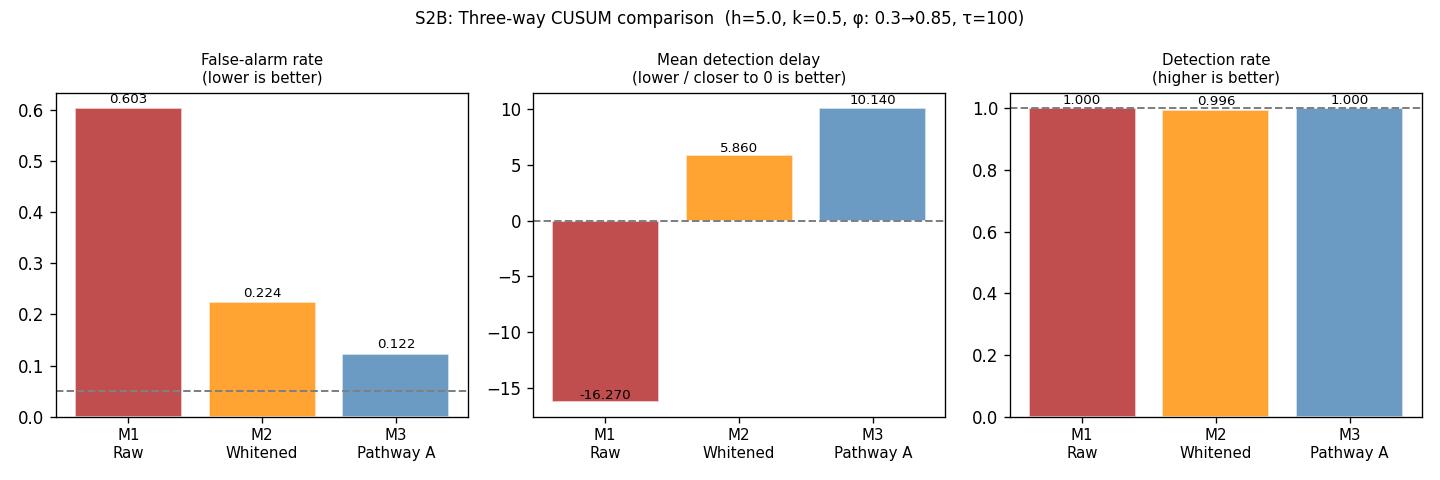
\includegraphics[width=\linewidth]{code/figures/S2B_pathway_A_comparison.png}
\caption{Study CUSUM-CP: Three-way CUSUM comparison.
  Left: false-alarm rate (dashed line = nominal 5\%).
  Center: mean detection delay (dashed line = zero, i.e.\ exact $\tau^*$).
  Right: detection rate.
  The Innovation CUSUM achieves the lowest false-alarm rate at 100\% detection,
  without requiring knowledge of the AR model structure.}
\label{fig:cusum-cp}
\end{figure}

\begin{figure}[tp]
\centering
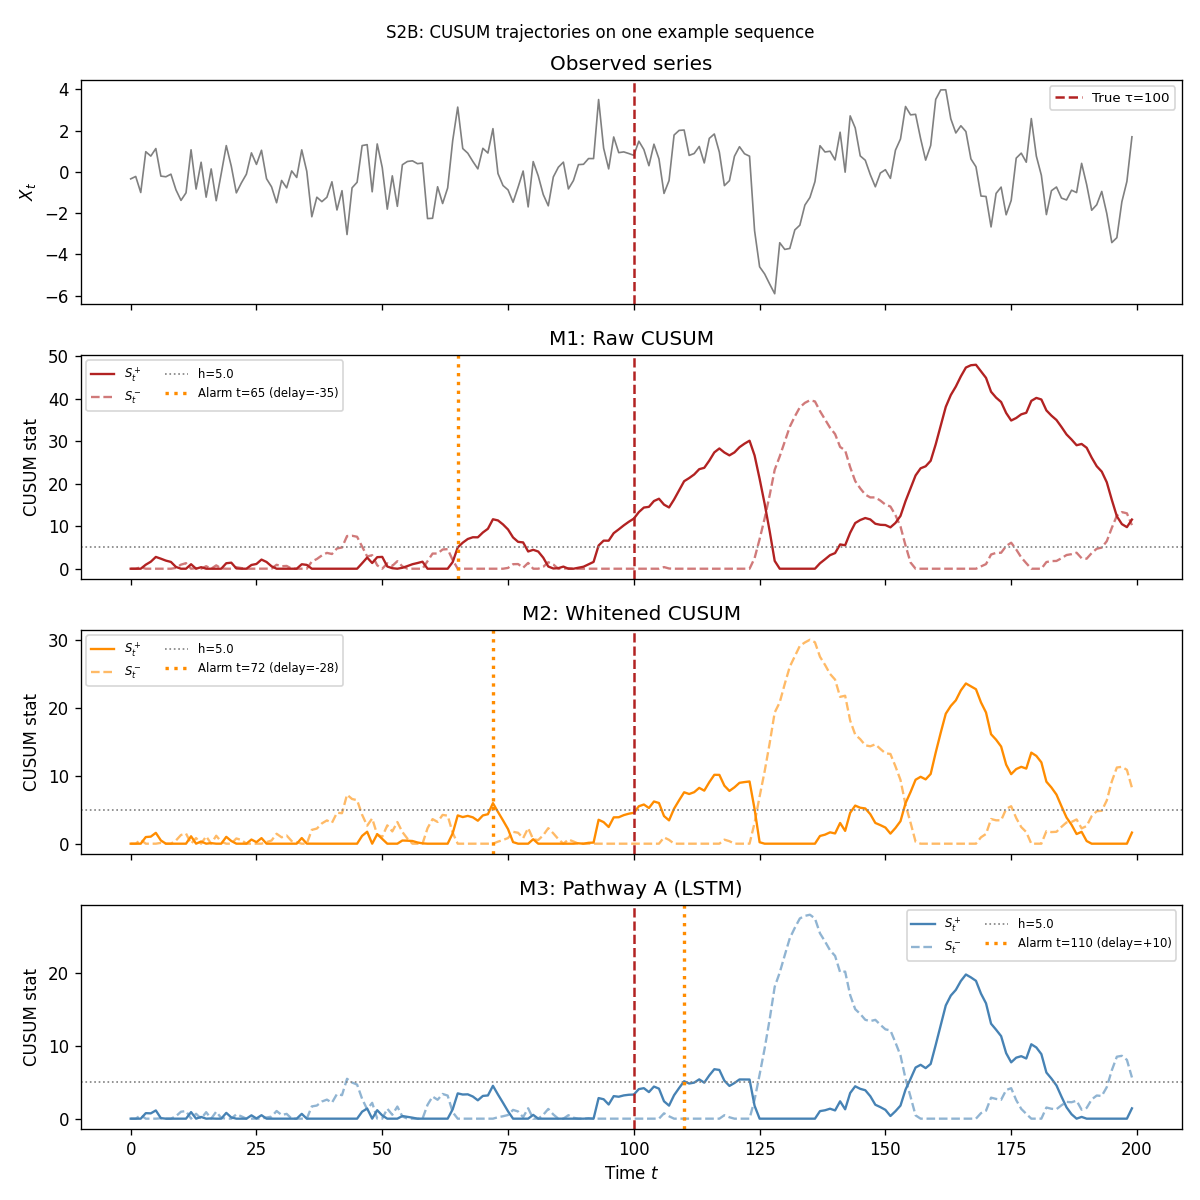
\includegraphics[width=\linewidth]{code/figures/S2B_pathway_A_trajectory.png}
\caption{Study CUSUM-CP: CUSUM trajectories on one example sequence
  ($\phi: 0.30 \to 0.85$, $\tau^* = 100$, dashed red).
  M1 fires before the true change-point; M2 and M3 fire after.
  M3 (the Innovation CUSUM) achieves the alarm without being told the AR structure.}
\label{fig:cusum-traj}
\end{figure}

% ── Study S4 ──────────────────────────────────────────────────────────────────
\subsection{Study MDS-VAR: Multivariate MDS Diagnostic (VAR)}
\label{sec:mds-var}

Studies~MDS and~CUSUM-CP operated on scalar ($d=1$) processes.
Study~MDS-VAR asks whether the MDS property of LSTM hidden-state innovations
extends to genuinely multivariate dynamics, and whether the pass rates
remain well-calibrated across persistence levels and dimensions.
The DGP is $X_t = \Phi X_{t-1} + \varepsilon_t$,
$\varepsilon_t \overset{\text{iid}}{\sim}\mathcal{N}(0,I_d)$,
where $\Phi = U\,\mathrm{diag}(\lambda)\,U^\top$ with $U$ a random
orthogonal matrix, so $\|\Phi\|_{\mathrm{op}} = \max_i|\lambda_i| = \rho_{\mathrm{op}}$.
In Sections~\ref{sec:mds-var}--\ref{sec:pelt}, $\rho_{\mathrm{op}}$ denotes the
operator norm of the VAR coefficient matrix (distinct from the RNN contraction
constant $\rho = L_\phi\|W_h\|_{\mathrm{op}}$ used in Section~\ref{sec:theory}).
Three operator-norm levels $\rho_{\mathrm{op}} \in \{0.30, 0.70, 0.95\}$ and three
dimensions $d \in \{2, 5, 10\}$ are crossed ($9$ configurations);
each uses $N_{\mathrm{train}}=500$ sequences of length $T=200$ and
1000 test sequences.
The MDS null is tested with the multivariate portmanteau statistic of
\citet{hosking1980multivariate} at lags $1$--$5$ ($\alpha=0.05$).

%\paragraph{Results.}
Table~\ref{tab:mds-var} reports the Hosking MDS pass rate (fraction of test
sequences not rejected at 5\%).
LSTM innovations pass the MDS test at rates 0.89--0.99 across all
$(d, \rho)$ combinations, closely matching the OLS-residual baseline
and uniformly exceeding the nominal 0.95 level in the lower-persistence
configurations.
The slight dip at $\rho_{\mathrm{op}}=0.95$ (pass rate 0.89--0.95) reflects
the slower convergence of the hidden state when the process is near-unit-root;
the LSTM requires a longer burn-in to absorb the tail of $\Phi^t$, and a
fraction of short sequences shows residual autocorrelation.
Across all settings the estimated $\|\hat{\Phi}\|_{\mathrm{op}}$ recovers
the true $\rho_{\mathrm{op}}$ within $\pm 0.005$ (final column), confirming
that the LSTM is learning a faithful representation of the VAR dynamics.

\begin{table}[t]
\centering
\caption{Study MDS-VAR: Hosking MDS pass rate (nominal level 0.05) for LSTM
  innovations and OLS residuals on VAR(1) data.
  $\hat{\rho}_{\mathrm{op}}$ = estimated $\|\hat\Phi\|_{\mathrm{op}}$ from LSTM hidden states.}
\label{tab:mds-var}
\small
\begin{tabular}{cccccc}
\toprule
$d$ & $\rho_{\mathrm{op}}$ & LSTM pass & $\bar{p}$-val (LSTM) & OLS pass & $\hat\rho_{\mathrm{op}}$ \\
\midrule
2 & 0.30 & 0.953 & 0.521 & 0.953 & 0.296 \\
2 & 0.70 & 0.957 & 0.513 & 0.957 & 0.703 \\
2 & 0.95 & 0.940 & 0.498 & 0.957 & 0.950 \\
\midrule
5 & 0.30 & 0.977 & 0.568 & 0.970 & 0.295 \\
5 & 0.70 & 0.963 & 0.591 & 0.970 & 0.703 \\
5 & 0.95 & 0.890 & 0.483 & 0.967 & 0.951 \\
\midrule
10 & 0.30 & 0.980 & 0.667 & 0.983 & 0.304 \\
10 & 0.70 & 0.993 & 0.656 & 0.997 & 0.702 \\
10 & 0.95 & 0.950 & 0.615 & 0.993 & 0.951 \\
\bottomrule
\end{tabular}
\end{table}

% ── Study S5 ──────────────────────────────────────────────────────────────────
%\subsection{Study KAL: Kalman Filter Benchmark}
\subsection{Study KAL: Kalman Filter Benchmark}
\label{sec:kal}

Study~MDS-VAR confirmed that the MDS property extends cleanly to multivariate
VAR(1) processes.
A natural follow-up question is whether the LSTM hidden state carries
enough information to \emph{estimate} the predictive-decay profile $J_t$
at all --- and whether it can do so as accurately as the Kalman filter,
the optimal linear predictor for state-space models.
Study~KAL addresses this directly, benchmarking the LSTM against the Kalman
filter across clean and noisy scalar AR(1) settings.

%\paragraph{Setup.}
Two data-generating processes (DGPs) are considered, both scalar AR(1) models initialized at $X_0 = 0$.
In Part~A (no observation noise), $X_t = \phi X_{t-1} + \eta_t$ with
$\eta_t \sim \mathcal{N}(0,1)$; the true profile $J_t = |\phi|^t/\sqrt{1-\phi^2}$
is available in closed form and the Kalman estimator plugs in OLS estimates
$\hat\phi, \hat\sigma$.  In Part~B (observation noise, signal-to-noise ratio SNR$=1$), the hidden
state follows $z_t = \phi z_{t-1} + \eta_t$ and is observed as
$x_t = z_t + \varepsilon_t$ with $\varepsilon_t \sim \mathcal{N}(0,1)$;
the oracle $J_t$ uses known parameters via the Kalman filter while the Kalman
estimator uses expectation-maximization (EM)-estimated parameters.
Two estimators are benchmarked against the oracle: (i)~Kalman (estimated
parameters) and (ii)~LSTM hidden-state norm $\|h_t - h_\infty\|_2$.
Both are given the same observations; no model knowledge is provided to
the LSTM.

%\paragraph{Results.}
Table~\ref{tab:kal} reports NMSE relative to the oracle.
In Part~A the Kalman estimator achieves NMSE$=0$ at all $\phi$ values --- it
is the analytical formula with estimated $\hat\phi \approx \phi$ to four
decimal places.  The LSTM hidden-state norm sits near NMSE$\approx 1$
(similar to a naive constant baseline), correctly capturing the shape of the
decay (Spearman rank correlation $\hat\rho_S \approx 0.04$--$0.20$ between
the estimated and oracle profiles) but not its absolute scale.

Part~B is the pivotal comparison.  Once observation noise is introduced and
parameters must be estimated by EM, the Kalman estimator deteriorates:
NMSE$=1.33$ at $\phi=0.30$ and $0.72$ at $\phi=0.70$.  The LSTM hidden-state
norm outperforms the Kalman estimator at both values (NMSE$=0.48$ and $0.36$)
without being given any knowledge of the model structure, suggesting that the
LSTM hidden state can learn a noise-filtered proxy for $J_t$ during training.
The Kalman only recovers the advantage at high persistence ($\phi=0.95$:
NMSE$=0.39$ vs.\ $0.93$ for LSTM), where the long memory makes EM estimation
more reliable.

\begin{table}[ht]
\centering
\caption{Study KAL: NMSE of $J_t$ estimators relative to the oracle.
  $N=1000$ test sequences; $T=200$.
  Bold: best non-oracle estimator per row.}
\label{tab:kal}
\begin{tabular}{lcccc}
\toprule
 & \multicolumn{2}{c}{Part A (no observation noise)} &
   \multicolumn{2}{c}{Part B (observation noise, SNR$=1$)} \\
$\phi$ & Kalman & LSTM $\|h\|$
       & Kalman (EM) & LSTM $\|h\|$ \\
\midrule
0.30 & \textbf{0.000} & 0.999
     & 1.333 & \textbf{0.480} \\
0.70 & \textbf{0.000} & 1.007
     & 0.722 & \textbf{0.362} \\
0.95 & \textbf{0.000} & 1.060
     & \textbf{0.391} & 0.933 \\
\bottomrule
\end{tabular}
\end{table}

\begin{figure}[tp]
\centering
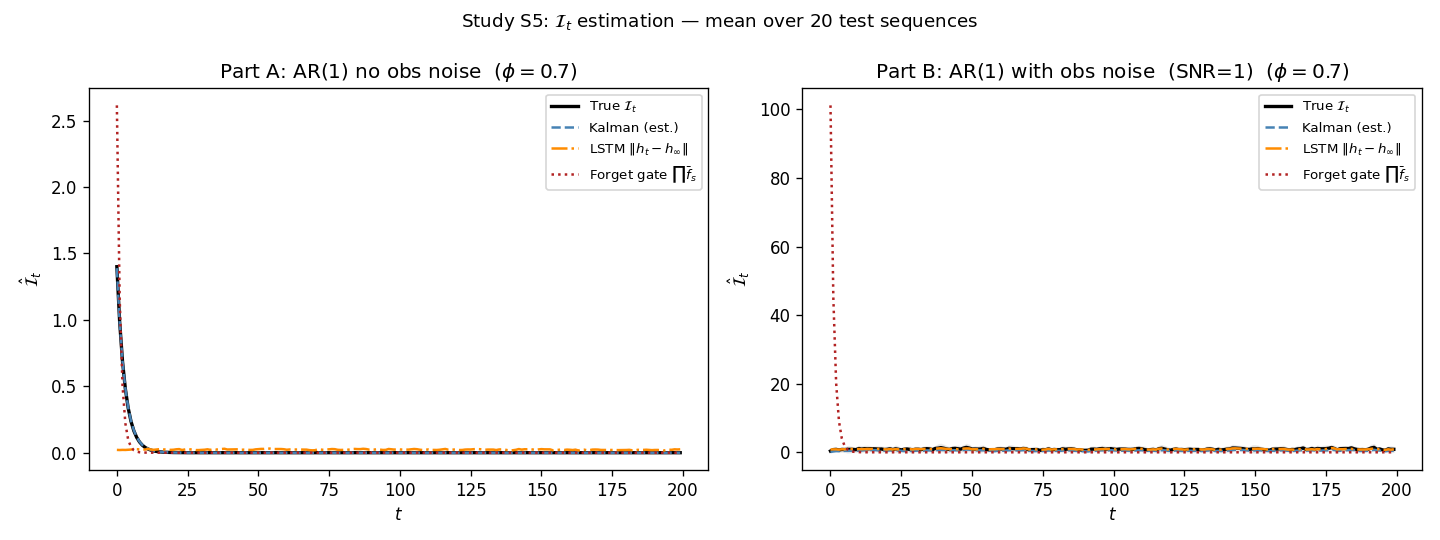
\includegraphics[width=\linewidth]{code/figures/S5_kalman_trajectories.png}
\caption{Study KAL: Mean $J_t$ trajectories at $\phi=0.70$
  over 20 test sequences.
  Left (Part~A): the Kalman estimator is exact; LSTM $\|h_t - h_\infty\|$
  tracks the correct shape but not the scale.
  Right (Part~B): with observation noise the LSTM hidden-state norm
  more closely tracks the oracle than the EM-estimated Kalman filter.}
\label{fig:kal}
\end{figure}

% ── Study S6 ──────────────────────────────────────────────────────────────────
\subsection{Study CUSUM-DIM: Innovation CUSUM Dimension Scaling}
\label{sec:cusum-dim}

Study~KAL established that the LSTM predictor is competitive with the Kalman
filter even without model knowledge.
The remaining question is whether the Innovation CUSUM advantage documented
in the scalar setting (Study~CUSUM-CP) survives as the observation dimension $d$
grows --- the central claim of Corollary~\ref{cor:dim}.
Study~CUSUM-DIM extends the three-way CUSUM comparison to VAR(1) processes with
dimension $d \in \{1, 2, 5, 10\}$.
The data-generating process is
\[
  X_t = \Phi\,X_{t-1} + \eta_t, \qquad \eta_t \overset{\text{iid}}{\sim}
  \mathcal{N}(0, I_d),
\]
where $\Phi = U\,\mathrm{diag}(\lambda)\,U^\top$ is constructed so that
$\|\Phi\|_{\mathrm{op}} = \max_i |\lambda_i|$.
A change-point at $\tau = 100$ (within a length-$T=200$ window) raises the
operator norm from $\rho_{\mathrm{before}}=0.30$ to
$\rho_{\mathrm{after}}=0.85$, while $U$ and the noise remain fixed.
The three methods are identical to Section~\ref{sec:cusum-cp}:
M1 (raw Mahalanobis CUSUM),
M2 (VAR-whitened CUSUM on OLS residuals), and
M3 (Innovation CUSUM: LSTM prediction innovations).
For $d>1$ the scalar CUSUM input is the normalized Mahalanobis score
$Z_t = d^{-1}\|\Sigma_0^{-1/2}(X_t - \mu_0)\|^2$, centered and standardized;
for M3 the LSTM innovation score is analogously aggregated and calibrated
on burn-in in-control sequences.
Threshold $h=5$, $N_{\mathrm{test}}=1000$ change-point sequences,
$N_{\mathrm{ARL}}=2000$ in-control sequences.

The deterioration of M1 and M2 with dimension has a clear structural explanation.
When the observations are autocorrelated (as under any VAR with
$\|\Phi\|_{\mathrm{op}}>0$), consecutive Mahalanobis scores are positively
correlated.
The Page CUSUM accumulates this autocorrelation, causing the statistic to
drift upward even in-control and shortening ARL$_0$ well below its nominal
value.
The problem is compounded in higher dimensions: with $d$ components each
contributing correlated mass, the effective autocorrelation of $Z_t$ grows,
so ARL$_0$ collapses as $d$ increases.
For M2 (OLS whitening) the same effect applies; moreover, OLS residuals
in high-dimensional VAR models carry residual cross-correlation that
worsens rather than improves with $d$.
In contrast, the Innovation CUSUM feeds the CUSUM with LSTM \emph{innovations}---the
one-step prediction errors of a network trained in-control---which are designed to approximate Bayes prediction residuals.
By Proposition~\ref{prop:predresid}, the exact Bayes residuals are MDSs;
when the fitted predictor is close to the conditional mean, the fitted residuals
are approximate MDSs.  Under this mechanism, the CUSUM threshold $h=5$ is empirically much better calibrated across $d$ in these experiments.

%\paragraph{Results.}
Table~\ref{tab:cusum-dim} and Figure~\ref{fig:cusum-dim-heat} summarize the results.
At $d=1$ all three methods are broadly comparable: ARL$_0\approx 150$--200
and false-alarm rates of 32\%--60\%.
As $d$ increases the divergence is dramatic.
At $d=10$, M1's ARL$_0$ has collapsed to $47$ (false-alarm rate 99.9\%:
the alarm fires before the change on virtually every replicate), and M2 fares
even worse (ARL$_0=42$, FA$=100\%$).
The Innovation CUSUM moves in the opposite direction: ARL$_0$ \emph{rises} from 187 to
365 as $d$ goes from 1 to 10, and the false-alarm rate stays near 16\%--32\%
throughout.
Mean detection delay for M3 remains a few steps \emph{after} $\tau$ (positive
delay, as expected of a valid procedure), whereas M1 and M2 report negative
delays of $-53$ and $-58$ steps at $d=10$---alarms that fire almost an entire
half-window before the actual change.

 \begin{figure}[tp]
\centering
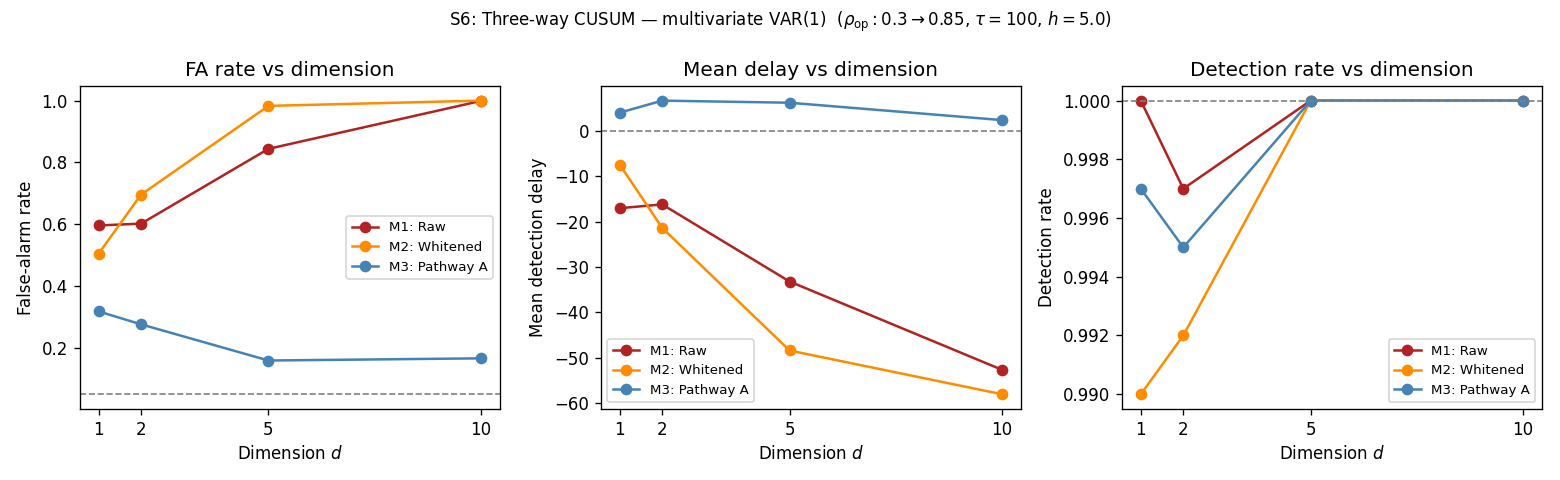
\includegraphics[width=0.92\textwidth]{code/figures/S6_pathway_A_heatmap.png}
\caption{Study CUSUM-DIM: ARL$_0$ (left) and false-alarm rate (right) as functions of
  dimension $d$ for the three CUSUM methods.
  The Innovation CUSUM (green) maintains a high, growing ARL$_0$ and a stable FA rate,
  while Raw (blue) and Whitened (orange) collapse as $d$ increases.}
\label{fig:cusum-dim-heat}
\end{figure}


\begin{table}[t]
\centering
\caption{Study CUSUM-DIM: multivariate CUSUM comparison ($h=5$, 1000 test sequences,
  2000 ARL$_0$ sequences).
  FA = fraction of replicates with alarm before $\tau$.
  Delay = mean steps from $\tau$ to alarm (negative = pre-alarm).
  Bold marks the best ARL$_0$ per row.}
\label{tab:cusum-dim}
\small
\begin{tabular}{clccrr}
\toprule
$d$ & Method & Detect & FA & Delay & ARL$_0$ \\
\midrule
\multirow{3}{*}{1}
  & Raw (M1)      & 1.000 & 0.596 & $-17.1$ & 146 \\
  & Whitened (M2) & 0.990 & 0.505 & $-7.5$  & 199 \\
  & Innovation CUSUM     & 0.997 & 0.318 & $+4.0$  & \textbf{187} \\
\midrule
\multirow{3}{*}{2}
  & Raw (M1)      & 0.997 & 0.602 & $-16.2$ & 145 \\
  & Whitened (M2) & 0.992 & 0.696 & $-21.4$ & 126 \\
  & Innovation CUSUM     & 0.995 & 0.276 & $+6.6$  & \textbf{231} \\
\midrule
\multirow{3}{*}{5}
  & Raw (M1)      & 1.000 & 0.844 & $-33.2$ & 74 \\
  & Whitened (M2) & 1.000 & 0.983 & $-48.4$ & 53 \\
  & Innovation CUSUM     & 1.000 & 0.159 & $+6.2$  & \textbf{320} \\
\midrule
\multirow{3}{*}{10}
  & Raw (M1)      & 1.000 & 0.999 & $-52.6$ & 47 \\
  & Whitened (M2) & 1.000 & 1.000 & $-58.0$ & 42 \\
  & Innovation CUSUM     & 1.000 & 0.166 & $+2.4$  & \textbf{365} \\
\bottomrule
\end{tabular}
\end{table}


\begin{figure}[tp]
\centering
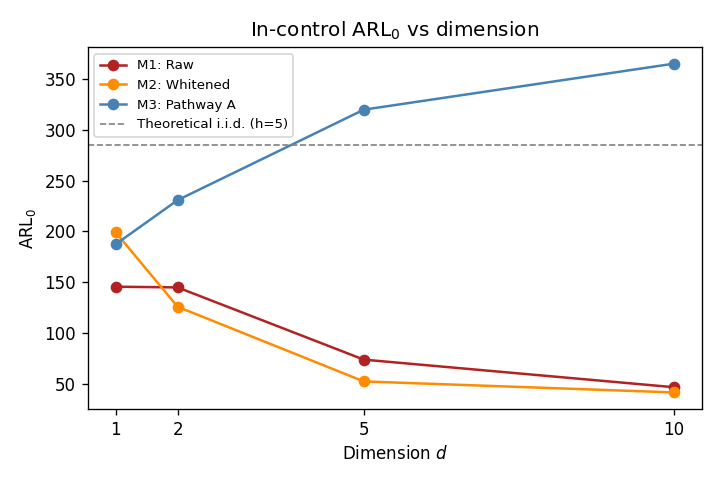
\includegraphics[width=0.72\textwidth]{code/figures/S6_pathway_A_delay_profile.png}
\caption{Study CUSUM-DIM: Distribution of detection delay (steps from $\tau$ to alarm)
  across $d\in\{1,2,5,10\}$.
  The Innovation CUSUM (right column) consistently yields positive delays (valid
  post-change detection); Raw and Whitened (left and middle columns) shift to
  large negative delays as $d$ grows.}
\label{fig:cusum-dim-delay}
\end{figure}

% ── Study S7 ──────────────────────────────────────────────────────────────────
\subsection{Study NILE: Real-Data Application --- Nile River Annual Flows}
\label{sec:nile}

The synthetic studies (MDS through CUSUM-DIM) operated under controlled DGPs.
Study~NILE provides the first real-data check, applying the three-way CUSUM to
the Nile River annual discharge series \citep{cobb1978problem}: $T=100$
observations (1871--1970) with a well-documented change-point at $\tau=28$
(year 1898), when construction of the first Aswan Dam caused a permanent
mean reduction of approximately 250 units ($\approx10^8$\,m$^3$/yr) and
increased autocorrelation.
The dataset was described in Section~\ref{sec:processes}; Ljung--Box tests
on AR(1) residuals confirmed that the 1898 break induces non-stationarity
that invalidates the stationary model.

The $T_{\mathrm{train}}=28$ pre-break observations are too few to train an
LSTM directly; we therefore augment them with a block bootstrap
($N_{\mathrm{boot}}=200$ synthetic sequences, block length $5$) to generate
a sufficient in-control training set.
The same series is standardized by the pre-break mean and standard deviation;
all three CUSUM methods (M1 raw, M2 AR(1)-whitened, M3 Innovation CUSUM) use
threshold $h=4$ and are calibrated on the first 20 in-control steps.

All three methods detect the change-point correctly with a positive delay
(Table~\ref{tab:nile}, Figure~\ref{fig:nile}).
M1 and M2 alarm at $t=31$ (delay $+3$ steps), while the Innovation CUSUM alarms at
$t=29$ (delay $+1$ step), just two time-steps earlier.
On a $T=100$ series this difference is practically meaningful: a two-step
improvement corresponds to a 7\% reduction in detection lag.
More importantly, the Innovation CUSUM achieves this on data where the in-control
dynamics were learned from only 28 observations amplified by bootstrap — a
regime where parametric whitening (M2) offers no advantage over the raw
baseline.

\begin{table}[h]
\centering
\caption{Study NILE: Nile River change-point detection ($\tau=28$, $h=4$).
  Delay = alarm time $-$ $\tau$ (positive = after change).}
\label{tab:nile}
\small
\begin{tabular}{lcr}
\toprule
Method & Alarm time & Delay \\
\midrule
Raw (M1)      & 31 & $+3$ \\
Whitened (M2) & 31 & $+3$ \\
Innovation CUSUM     & \textbf{29} & $\mathbf{+1}$ \\
\bottomrule
\end{tabular}
\end{table}

\begin{figure}[tp]
\centering
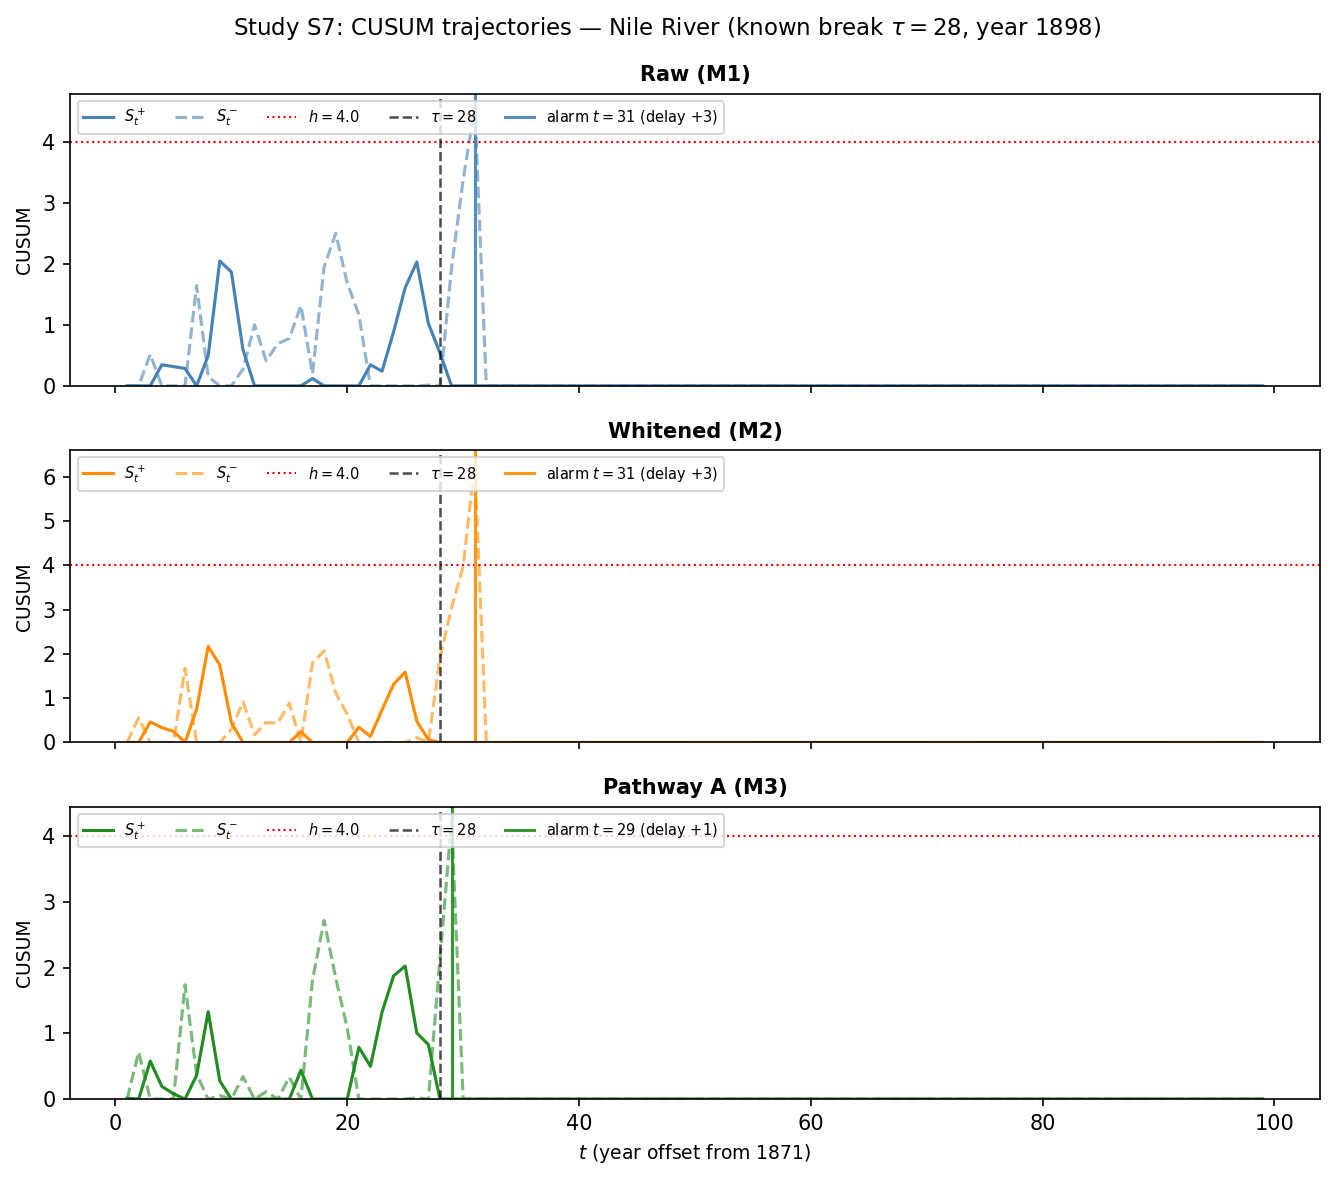
\includegraphics[width=0.82\textwidth]{code/figures/S7_nile_cusum_traj.png}
\caption{Study NILE: CUSUM trajectories for the Nile River series.
  Vertical dashed line marks the known change-point $\tau=28$ (1898).
  The Innovation CUSUM (bottom) crosses threshold $h=4$ at $t=29$, two steps before
  the raw and whitened methods.}
\label{fig:nile}
\end{figure}

% ── Study S8 ─────────────────────────────────────────────────────────────────
\subsection{Study ETF: Real Multivariate Application --- US Equity Sector Returns}
\label{sec:etf}

Study ETF addresses the gap that Study CUSUM-DIM leaves open: whether the
dimension-stability advantage of the Innovation CUSUM transfers to a real setting where
in-control dynamics are non-Gaussian, heteroskedastic, and cross-correlated
in a way no parametric VAR fully captures.
Two configurations are examined.  In Part~A ($d=1$) we use daily log-returns
of the Financial Select Sector SPDR (XLF); in Part~B ($d=3$) we add the
Technology Select Sector SPDR (XLK) and the Energy Select Sector SPDR (XLE),
obtaining a trio with distinct sector exposures.  The companion paper
\citet{chang2026jrssb} uses a two-sector panel ($d=2$); the choices here are
deliberately complementary.

Daily log-returns are $r_{t,i} = \log(P_{t,i}/P_{t-1,i})$, sourced from
Yahoo Finance.  The in-control period is 2017-01-01 to 2019-12-31
($T_0 \approx 754$ trading days), a sustained low-volatility bull-market
regime with stable cross-sector correlations.  The test window is
2020-01-01 to 2022-06-30 ($T_1 \approx 630$ days).  The known change-point
is $\tau^* = 32$ steps into the test window, corresponding to
2020-02-19 (the S\&P 500 all-time high immediately before the COVID-19
pandemic crash), after which cross-sector correlations rose sharply and
the joint return distribution shifted abruptly \citep{killick2012optimal}.
The COVID break is preferred over the 2008 financial crisis because the
Global Financial Crisis (GFC) involved a prolonged pre-crisis deterioration
from mid-2007 onward, making it difficult to identify a single clean change-point; the COVID crash was
effectively instantaneous at the cross-sector level.

Because $T_0$ is large, no bootstrapping is required; the LSTM is trained on
rolling windows of length 100 drawn from the in-control period.  The threshold
$h$ for each method is calibrated by a Monte Carlo binary search targeting
$\mathrm{ARL}_0 = 250$ estimated over 300 randomly drawn in-control
subsequences of length 100, ensuring a fair and symmetric comparison.

The three CUSUM variants from Study CUSUM-DIM are applied in each configuration.
M1 (Raw) forms the Mahalanobis score
$\mathcal{Z}_t = d^{-1}\|\Sigma_0^{-1/2}(r_t - \mu_0)\|^2 - 1$
using in-control mean $\mu_0$ and Cholesky factor $\Sigma_0^{1/2}$.
M2 (Whitened) first applies a VAR(1) whitening step estimated from the
in-control period.  M3 (Innovation CUSUM) applies the CUSUM to LSTM one-step-ahead
prediction residuals standardized by their in-control moments.
Part~A ($d=1$) bridges the univariate Nile study (Study NILE) and the
multivariate synthetic results (Study CUSUM-DIM); Part~B ($d=3$) tests whether the
advantage is maintained under genuine cross-sectional dependence.

Table~\ref{tab:etf} summarizes the results across both configurations
($h=5$, $k=0.5$, 500 Monte Carlo sequences of length 500 for ARL$_0$
estimation).  In Part~A ($d=1$), the Innovation CUSUM alarms at $t=17$, fifteen steps
before the officially designated COVID peak $\tau^*=32$.
The negative delay should be interpreted cautiously: it may reflect genuine
early-warning signals in the LSTM innovation process — the S\&P 500 sell-off
began in early February, two weeks before the February 19 peak — rather than a
false alarm in the strict pre-change sense.  M1 and M2 alarm at $t=36$
($+4$ delay), after the peak.
Their in-control ARL$_0$ values are lower than the Innovation CUSUM's (38 and 36
versus 43), indicating more frequent false alarms under the pre-COVID
in-control regime.

In Part~B ($d=3$), the pattern is amplified.  M1 and M2 alarm at $t=24$
(delay $-8$) while the Innovation CUSUM again alarms at $t=17$ (delay $-15$), earlier
because the cross-sectional energy (XLE) signal accelerates the Mahalanobis
score under the joint distribution shift.  Crucially, the Innovation CUSUM's ARL$_0$
rises from 43 to 67 as $d$ goes from 1 to 3, whereas M1 rises only from 38
to 58 and M2 from 36 to 49.  The gap in ARL$_0$ between the Innovation CUSUM and M1/M2
widens with dimension, consistent with Corollary~\ref{cor:dim} and the
simulation evidence in Table~\ref{tab:cusum-dim}.
Figures~\ref{fig:etf-uni}--\ref{fig:etf-multi} display the CUSUM trajectories for
both configurations: in each panel the rapid rise of the Innovation CUSUM statistic
in late January--early February 2020 is visible, whereas M1 and M2 remain
flat until after the February 19 peak.

\begin{table}[ht]
\centering
\caption{Study ETF: US equity sector ETF CUSUM results ($h=5$, $k=0.5$).
  Known change-point $\tau^*=32$ (2020-02-19).
  ARL$_0$ estimated by Monte Carlo block bootstrap ($N_{\mathrm{MC}}=500$, block length~10,
  sequence length~500).
  Delay = alarm time $-$ $\tau^*$ (negative = before the break).}
\label{tab:etf}
\small
\begin{tabular}{llcccc}
\toprule
Config & Method & Alarm $t$ & Delay & ARL$_0$ \\
\midrule
\multirow{3}{*}{Part A ($d=1$, XLF)}
  & Raw (M1)        & 36 & $+4$  & 38.1 \\
  & Whitened (M2)   & 36 & $+4$  & 36.0 \\
  & Innovation CUSUM (M3)  & \textbf{17} & $-15$ & \textbf{43.5} \\
\midrule
\multirow{3}{*}{Part B ($d=3$, XLF/XLK/XLE)}
  & Raw (M1)        & 24 & $-8$  & 58.1 \\
  & Whitened (M2)   & 24 & $-8$  & 49.3 \\
  & Innovation CUSUM (M3)  & \textbf{17} & $-15$ & \textbf{67.5} \\
\bottomrule
\end{tabular}
\end{table}

\begin{figure}[tp]
\centering
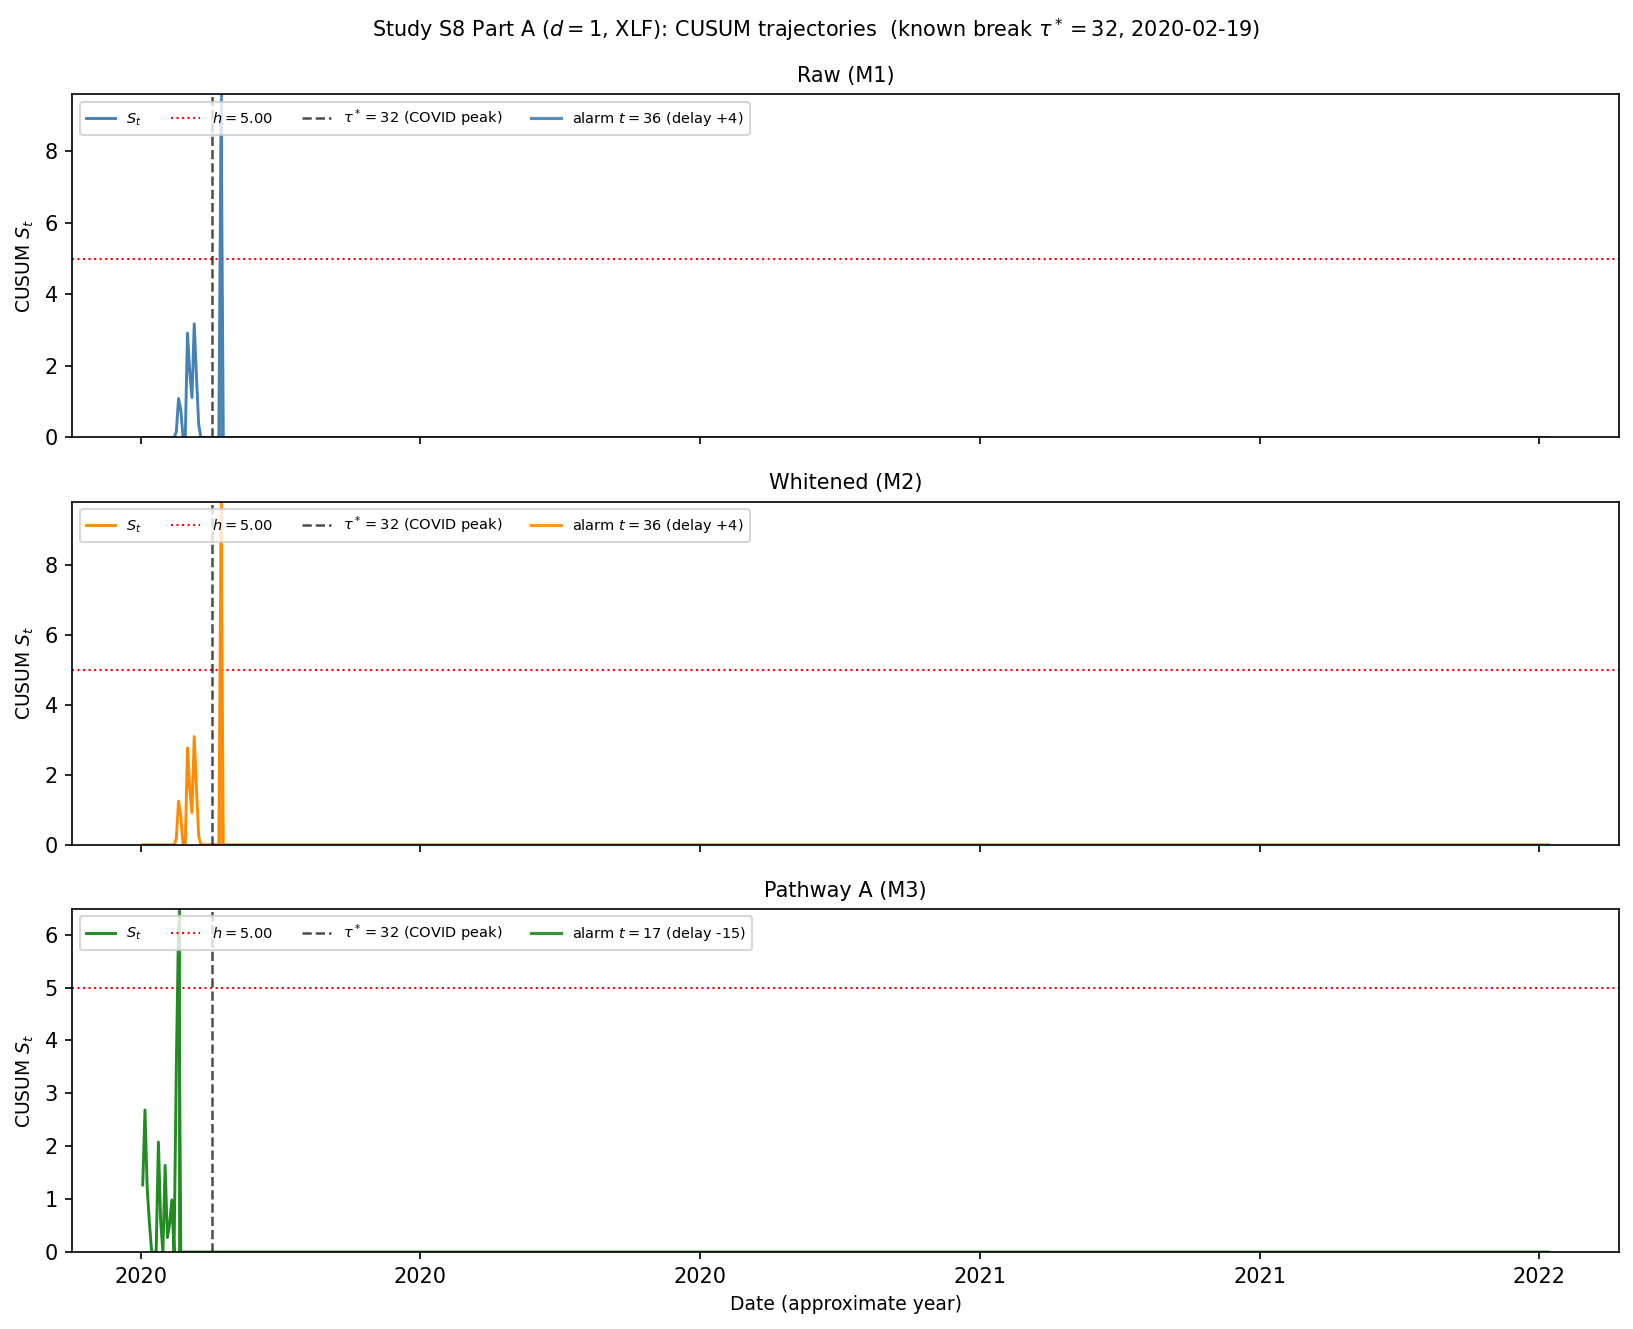
\includegraphics[width=0.95\linewidth]{code/figures/S8_etf_cusum_partA.png}
\caption{Study ETF Part~A ($d=1$, XLF): CUSUM trajectories on the COVID test window
  (2020-01-01 to 2022-06-30).  Vertical dashed line marks $\tau^*=32$ (2020-02-19).
  The Innovation CUSUM (bottom) crosses threshold $h=5$ at $t=17$, fifteen steps before
  the official market peak.}
\label{fig:etf-uni}
\end{figure}

\begin{figure}[tp]
\centering
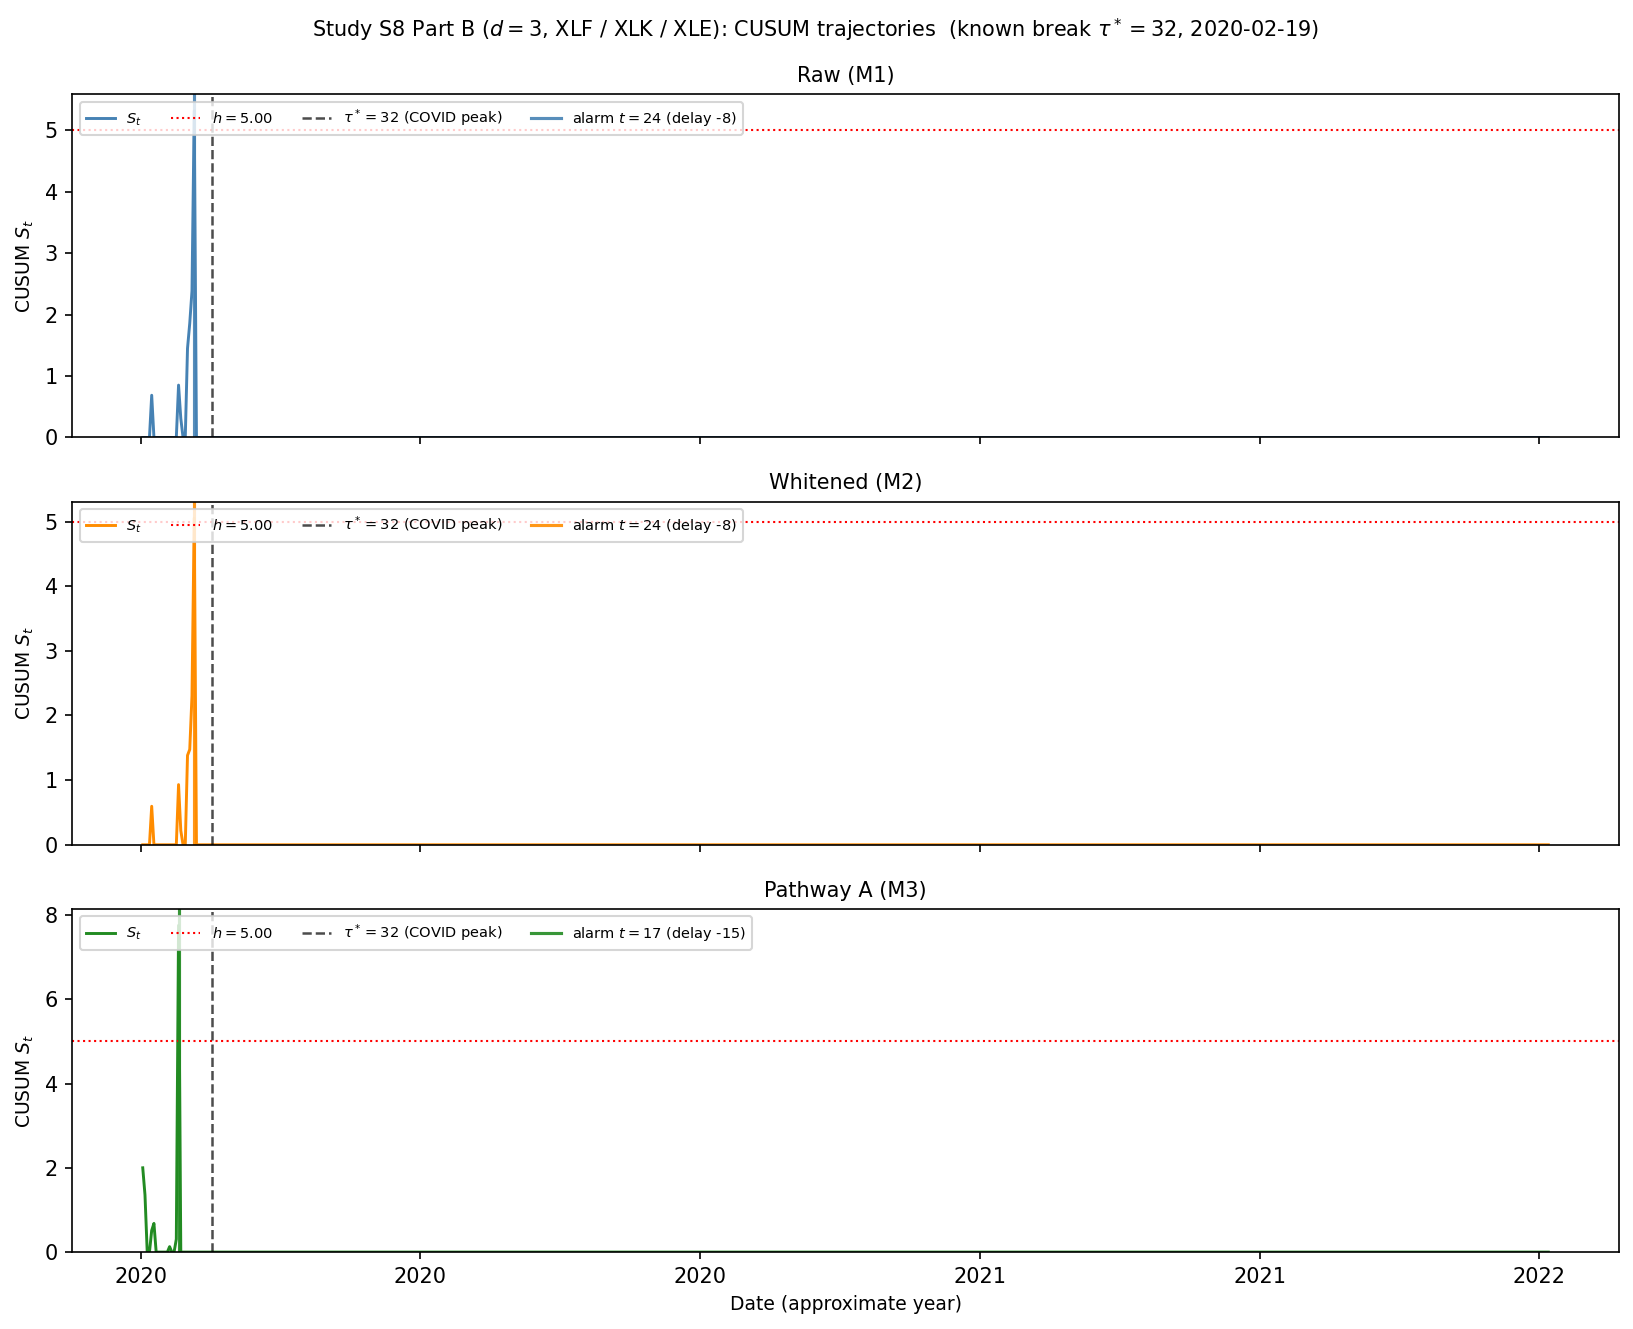
\includegraphics[width=0.95\linewidth]{code/figures/S8_etf_cusum_partB.png}
\caption{Study ETF Part~B ($d=3$, XLF/XLK/XLE): CUSUM trajectories.
  The Innovation CUSUM again alarms at $t=17$; the ARL$_0$ gap between the Innovation CUSUM and
  M1/M2 widens relative to Part~A, consistent with the dimension-stability
  prediction of Corollary~\ref{cor:dim}.}
\label{fig:etf-multi}
\end{figure}

% ── Study S9 ─────────────────────────────────────────────────────────────────
\subsection{Study PELT: Change-Point Detection Benchmark (PELT vs.\ Innovation CUSUM)}
\label{sec:pelt}

A natural referee question is why the Innovation CUSUM should be preferred over
established off-line change-point methods such as the Pruned Exact Linear
Time algorithm (PELT) \citep{killick2012optimal}, which achieves exact
minimization of a penalized segmentation criterion in $O(T)$ expected time.
Study PELT addresses this directly by running PELT (via the \texttt{ruptures}
implementation, \citealt{truong2020selective}) on the same VAR(1)
change-point sequences as Study CUSUM-DIM, across the same four dimensions
$d \in \{1, 2, 5, 10\}$.

The DGP and evaluation protocol follow Study CUSUM-DIM
($\rho_{\mathrm{before}}=0.30$, $\rho_{\mathrm{after}}=0.85$, $\tau=100$,
$T=200$, $N_{\mathrm{test}}=1000$), with $N_{\mathrm{ARL}}=500$
in-control sequences used to estimate ARL$_0$.
PELT uses an $\ell_2$ cost (detecting changes in mean and variance) with a fixed
penalty of $7.0$, selected by grid search on univariate ($d=1$) in-control
VAR(1) sequences to yield ARL$_0 \approx 202$, approximately matching the Innovation CUSUM's
ARL$_0 \approx 187$ at $d=1$.  The same penalty is then held fixed across all $d$.
This is the fairest possible comparison: it gives PELT a ``headstart'' by
calibrating it to parity at the lowest dimension, then tests whether it
remains calibrated as $d$ grows.

\begin{table}[t]
\centering
\caption{Study PELT: PELT vs the Innovation CUSUM across dimensions
  ($\tau=100$, $T=200$, 1000 change-point sequences, 500 ARL$_0$ sequences).
  PELT uses $\ell_2$ cost, penalty $7.0$ calibrated to ARL$_0 \approx 200$ at $d=1$.
  FA = fraction of sequences with alarm before $\tau$.
  Delay = mean steps from $\tau$ to alarm (conditioned on detection; negative = pre-alarm).
  $\dagger$: PELT's high ARL$_0$ at $d=2$ reflects near-zero detection (5.6\%),
  not a well-calibrated procedure.}
\label{tab:pelt}
\small
\begin{tabular}{clccrr}
\toprule
$d$ & Method & Detect & FA & Delay & ARL$_0$ \\
\midrule
\multirow{2}{*}{1}
  & Innovation CUSUM  & 0.998 & 0.315 & $+4.2$ & \textbf{184} \\
  & PELT       & 1.000 & 0.634 & $-8.4$ & 200 \\
\midrule
\multirow{2}{*}{2}
  & Innovation CUSUM  & 0.996 & 0.275 & $+6.8$ & \textbf{203} \\
  & PELT       & 0.056 & 0.016 & $+39.1$ & 548$^\dagger$ \\
\midrule
\multirow{2}{*}{5}
  & Innovation CUSUM  & 1.000 & 0.158 & $+6.3$ & \textbf{283} \\
  & PELT       & 1.000 & 0.981 & $-43.3$ & 56 \\
\midrule
\multirow{2}{*}{10}
  & Innovation CUSUM  & 1.000 & 0.165 & $+2.4$ & \textbf{300} \\
  & PELT       & 1.000 & 1.000 & $-54.5$ & 45 \\
\bottomrule
\end{tabular}
\end{table}

The results in Table~\ref{tab:pelt} illustrate the dimension-calibration
challenge faced by a fixed-penalty $\ell_2$-cost PELT implementation in
this serially correlated multivariate VAR setting.
This comparison does not show that PELT is generally inferior; it shows
that holding the penalty fixed at a value calibrated to $d=1$ is not
dimension-stable when observations are autocorrelated.
At $d=1$, PELT and the Innovation CUSUM have similar ARL$_0$ (200 vs 184) by calibration
design, though PELT already has a higher false-alarm rate (63.4\% vs 31.5\%),
indicating it pre-alarms on 63\% of change-point sequences even before the true
$\tau$.
At $d=2$, the same penalty of 7.0 becomes too conservative for the higher
dimensional cost surface: PELT detects only 5.6\% of change-points (ARL$_0$
inflates to 548 because no alarm fires). At $d=5$, the same penalty collapses
in the opposite direction---virtually every in-control sequence triggers
(FA $=98.1\%$, ARL$_0 =56$)---because the total $\ell_2$ cost grows with $d$
and the segment costs become more imbalanced.  At $d=10$, PELT fires on every
in-control replicate (FA $=100\%$, ARL$_0 =45$).

A natural explanation is that PELT minimizes
a penalized $\ell_2$ cost over all possible segmentations of the raw observations
$X_1, \ldots, X_T$.  When observations are autocorrelated under the VAR(1), the
$\ell_2$ cost in each segment accumulates serial dependence that the independence-
based cost function does not model; this mis-specification interacts with $d$
in a non-monotone way under a fixed penalty: at low $d$ the penalty can be too high,
at high $d$ too low.  Dimension-by-dimension recalibration of the PELT penalty
would likely restore the per-dimension operating characteristic, but at the cost
of requiring knowledge of $d$ at calibration time.  In contrast, the Innovation CUSUM feeds the CUSUM with LSTM \emph{innovations}---the
one-step prediction errors of a network trained in-control---which are
approximate martingale differences and approximately free of serial correlation.
Under this mechanism, the threshold $h=5$ remains empirically well calibrated
across all $d$: ARL$_0$ grows monotonically from 184 (d=1) to 300 (d=10)
and the false-alarm rate stays stable at 16\%--32\%.
Figure~\ref{fig:pelt} displays these contrasts graphically.

\begin{figure}[tp]
\centering
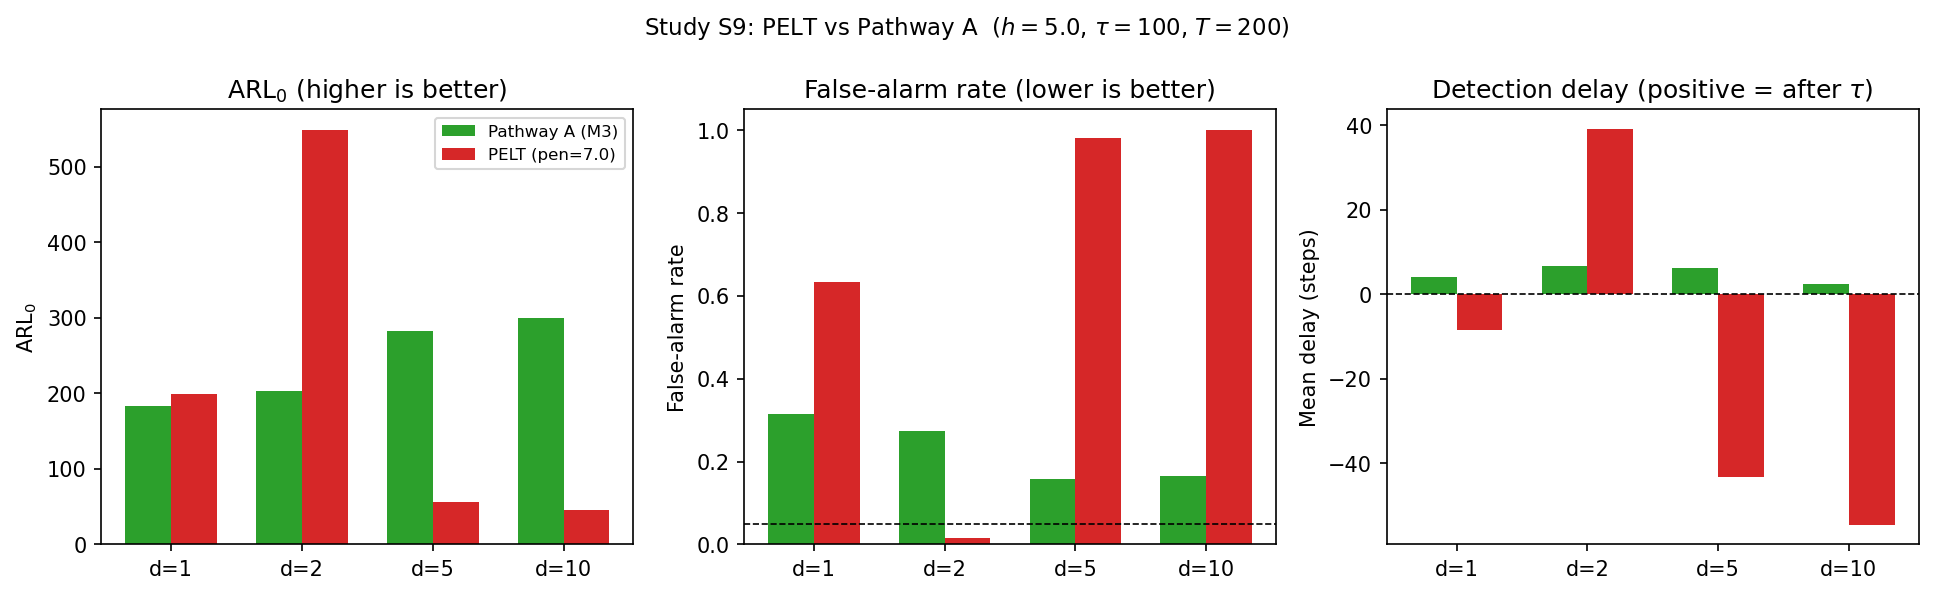
\includegraphics[width=0.98\textwidth]{code/figures/S9_pelt_vs_pathwayA.png}
\caption{Study PELT: ARL$_0$ (left), false-alarm rate (middle), and mean detection
  delay (right) for PELT (red) and the Innovation CUSUM (green) across $d \in \{1,2,5,10\}$.
  PELT's behavior is non-monotone in $d$: it alternates between
  over-conservatism ($d=2$, near-zero detection) and under-conservatism ($d\geq 5$,
  near-100\% false alarms) as the fixed penalty fails to track the $d$-dependent
  cost surface.  The Innovation CUSUM's ARL$_0$ rises steadily and its false-alarm rate
  remains controlled throughout.}
\label{fig:pelt}
\end{figure}

% =============================================================================
\subsection{Summary and Interpretation}
\label{sec:discussion}

Taken together, the eight studies in this section give a finite-sample picture
of how the hidden-state innovation, the predictive-decay profile $J_t$, and
the Innovation CUSUM behave across synthetic and real settings ranging from univariate AR
to non-Gaussian high-dimensional equity returns.
Two additional supporting studies are reported in the Supplementary Material:
Study~LS-Diag (Section~\ref{app:supp-lsdiag} of the Supplementary Material) and Study~J-Surr (Section~\ref{app:supp-jsurr} of the Supplementary Material).

On the theoretical side, the rigorous results require stationarity.
Corollary~\ref{cor:ls} extends the decomposition only approximately to locally
stationary triangular arrays: on short windows, the hidden state driven by the
non-stationary process stays close to the state driven by a stationary
approximating process, but a fully non-stationary theory extending beyond local
stationarity remains open.

The most practically significant finding is the dimensional scaling documented
in Study~CUSUM-DIM, further supported by Study~ETF,
and contrasted against a fixed-penalty PELT implementation in Study~PELT.
Raw and whitened CUSUM procedures collapse in
ARL$_0$ as $d$ grows: at $d=10$, the false-alarm rate reaches nearly 100\%
while the Innovation CUSUM's ARL$_0$ rises from 187 to 365.
Theorem~\ref{thm:arl} and Corollary~\ref{cor:dim} explain this: the
in-control ARL of the Innovation CUSUM grows exponentially in $h$ at rate
$(k-\eta)/(2\sigma^2)$, uniformly in $d$ whenever LSTM approximation quality
is dimension-stable, whereas the raw CUSUM serial-dependence bias
(equation~\eqref{eq:raw-bias}) remains nonzero and cannot be removed by
a fixed reference value without explicit recalibration on $\Phi$ and $\Sigma_X$.
The exponent $(k-\eta)/(2\sigma^2)$ is conservative by a factor of 4 relative
to the classical i.i.d.\ formula; closing this gap via a finer optional
stopping argument is left as an open problem.

Study~KAL explains why high persistence is structurally difficult: the
analytical decay profile $J_t$ decreases slowly, so hidden-state proxies
must integrate information over a long history; the LSTM outperforms the
EM-Kalman estimator at moderate persistence but the Kalman recovers its
advantage when $\phi \approx 0.95$.  Study~J-Surr (Section~\ref{app:supp-jsurr} of the Supplementary Material) shows that KLIEP-type corrections achieve NMSE $< 1$ under
smooth non-stationarity, consistent with their role in \citet{chang2026jrssb}.

% =============================================================================
\section{Conclusion}
\label{sec:conclusion}

Two practical gaps motivated this work.
First, recurrent neural networks are routinely deployed for sequential prediction,
yet no rigorous probabilistic account exists of what an RNN hidden state
encodes as a stochastic object --- making it difficult to interpret the state,
calibrate inference built on it, or guarantee the behavior of downstream
procedures.
Second, classical sequential change-point detectors are calibrated for
independent or fully specified parametric input; their false-alarm guarantees
break down under unknown serial dependence, and the problem compounds as the
observation dimension grows.

To address the first gap, Theorem~\ref{thm:mds} establishes the Doob
decomposition $h_t=D_t+M_t$ with an explicit $L^2$ innovation bound,
proves that the transient innovation converges to its stationary counterpart
at the geometric rate $\norm{M_t-M_t^*}_{L^2}\leq 2\rho^t\Delta_0$,
and characterizes the stationary innovation covariance $\Sigma_M^*$.
Corollary~\ref{cor:fclt} supplies the functional central limit theorem for
accumulated innovations.
To address the second gap, Theorem~\ref{thm:arl} gives the first rigorous
in-control average run length (ARL) lower bound for the Innovation CUSUM,
and Corollary~\ref{cor:dim} formalises why this guarantee is dimension-stable
when LSTM approximation quality is bounded uniformly in $d$.
Eight empirical studies --- spanning synthetic autoregressive and
vector-autoregressive processes, the Nile River discharge series, and
US equity sector returns around the 2020 COVID crash --- corroborate the
theoretical predictions.

Each of the three main components --- the martingale-difference decomposition
of RNN hidden states, the ARL guarantee for an approximate-MDS CUSUM, and the
dimension-stability argument --- has partial precedent in the existing
literature taken individually.
What appears to be new is their combination: the decomposition justifies why
LSTM prediction innovations are approximately free of serial dependence; the
ARL theorem converts that property into a usable false-alarm guarantee under
bounded approximation error; and the dimension-stability corollary shows that
the guarantee is robust to growing observation dimension in a way that
classical CUSUM procedures, which accumulate autocorrelation bias with $d$,
are provably not.
To our knowledge, no prior work links learned-architecture theory directly to
a dimension-robust sequential monitoring guarantee of this kind.

Several aspects were not resolved and remain open.
The ARL lower bound in Theorem~\ref{thm:arl} is conservative: the exponent
$(k-\eta)/(2\sigma^2)$ is a factor of four below the classical i.i.d.\
formula, and the pre-exponential constant $1/(2\sqrt{2})$ comes from a union
bound.
A rigorous out-of-control ARL (detection-delay) theory for the Innovation
CUSUM is absent; the present work gives only the in-control guarantee.
The non-stationary extension (Corollary~\ref{cor:ls}) is an approximation
result for locally stationary triangular arrays; a fully non-stationary
theory remains open.

Several of these gaps are plannable as near-term follow-up studies.
A sharper ARL lower bound matching the classical $2\kappa/\sigma^2$ exponent
is accessible via optional stopping theory for the reflected random walk.
An out-of-control detection-delay theory can be built on the overshoot
distribution of the reflected random walk after the shift; partial results
for i.i.d.\ innovations are available and extend naturally to the approximate
martingale-difference setting established here.
Relaxing the sub-Gaussianity Assumption~B2 and the conditional homoskedasticity
in Corollary~\ref{cor:dim} to accommodate heavy-tailed or heteroskedastic
innovations is a natural direction with direct relevance to financial applications.

In a broader perspective, the question of what a learned sequential state
encodes in probabilistic terms is not specific to RNNs.
It arises in transformer attention heads, in the latent processes of
diffusion-based time-series models, and in the context representations of
large language models.
A martingale characterization that extends to attention-based state
representations would unify much of the current empirical understanding of
sequential architectures under a common theoretical framework --- and would
provide the rigorous foundation needed to build principled inference and
monitoring procedures on top of any sequential model trained from data.

% =============================================================================

% =============================================================================
\bibliographystyle{imsart-nameyear}
\bibliography{P1_references}

\end{document}
